\documentclass[12pt,spanish,fleqn,openany,letterpaper,pagesize]{scrbook}

\usepackage[utf8]{inputenc}
\usepackage[spanish]{babel}%escribir con acentos sin necesidad de comandos \'{} .
\usepackage{fancyhdr}
\usepackage{epsfig}
\usepackage{epic}
\usepackage{eepic}
\usepackage{amsmath}
\usepackage{threeparttable}
\usepackage{amscd}
\usepackage{here}
\usepackage{graphicx}
\usepackage{lscape}
\usepackage{tabularx}
\usepackage{subfigure}
\usepackage{longtable}
\usepackage{multirow}
\usepackage{booktabs}
\usepackage{rotating}
\usepackage{tablefootnote}

\usepackage[colorinlistoftodos]{todonotes}


\usepackage{rotating} %Para rotar texto, objetos y tablas seite. No se ve en DVI solo en PS. Seite 328 Hundebuch
                        %se usa junto con \rotate, \sidewidestable ....


\renewcommand{\theequation}{\thechapter-\arabic{equation}}
\renewcommand{\thefigure}{\textbf{\thechapter-\arabic{figure}}}
\renewcommand{\thetable}{\textbf{\thechapter-\arabic{table}}}


\pagestyle{fancyplain}%\addtolength{\headwidth}{\marginparwidth}
\textheight22.5cm \topmargin0cm \textwidth16.5cm
\oddsidemargin0.5cm \evensidemargin-0.5cm%
\renewcommand{\chaptermark}[1]{\markboth{\thechapter\; #1}{}}
\renewcommand{\sectionmark}[1]{\markright{\thesection\; #1}}
\lhead[\fancyplain{}{\thepage}]{\fancyplain{}{\rightmark}}
\rhead[\fancyplain{}{\leftmark}]{\fancyplain{}{\thepage}}
\fancyfoot{}
\thispagestyle{fancy}%


\addtolength{\headwidth}{0cm}
\unitlength1mm %Define la unidad LE para Figuras
\mathindent0cm %Define la distancia de las formulas al texto,  fleqn las descentra
\marginparwidth0cm
\parindent0cm %Define la distancia de la primera linea de un parrafo a la margen

%Para tablas,  redefine el backschlash en tablas donde se define la posici\'{o}n del texto en las
%casillas (con \centering \raggedright o \raggedleft)
\newcommand{\PreserveBackslash}[1]{\let\temp=\\#1\let\\=\temp}
\let\PBS=\PreserveBackslash

%Espacio entre lineas
\renewcommand{\baselinestretch}{1.1}

%Neuer Befehl f\"{u}r die Tabelle Eigenschaften der Aktivkohlen
\newcommand{\arr}[1]{\raisebox{1.5ex}[0cm][0cm]{#1}}

%Neue Kommandos
\usepackage{Befehle}
%Inicio del documento. Tener en cuenta que hay archivos auxiliares

\begin{document}
\pagenumbering{roman}
%\newpage
%\setcounter{page}{1}
\begin{center}
\begin{figure}
\centering%

\epsfig{file=HojaTitulo/EscudoUN,scale=1}%
\end{figure}
\thispagestyle{empty} \vspace*{2.0cm} \textbf{\huge
Modelo Basado en el Contexto y la Semántica de Contenidos Multimodales
para Sistemas Sensibles al Contexto}\\[6.0cm]
\Large\textbf{Cristian Andrés Narváez Alarcón}\\[6.0cm]
\small Universidad Nacional de Colombia\\
Facultad de Ingeniería, Departamento de Ingeniería de Sistemas e Industrial\\
Bogotá, Colombia\\
2018\\
\end{center}

\newpage{\pagestyle{empty}\cleardoublepage}

\newpage
\begin{center}
\thispagestyle{empty} \vspace*{0cm} \textbf{\huge
Modelo Basado en el Contexto y la Semántica de Contenidos Multimodales}\\[3.0cm]
\Large\textbf{Cristian Andrés Narváez Alarcón}\\[3.0cm]
\small Tesis de grado presentada como requisito parcial para optar al
t\'{\i}tulo de:\\
\textbf{Magister en Ingenieria de Sistemas y Computación}\\[2.5cm]
Director(a):\\
Ph.D. Marcela Iregui Guerrero\\[2.0cm]
Co-director(a):\\
Ph.D. (opt) Denisse Cangrejo Aljure\\[2.0cm]
L\'{\i}nea de Investigaci\'{o}n:\\
Nombrar la l\'{\i}nea de investigaci\'{o}n en la que enmarca la tesis  o trabajo de investigaci\'{o}n\\
Grupo de Investigaci\'{o}n:\\
Nombrar el grupo en caso que sea posible\\[2.5cm]
Universidad Nacional de Colombia\\
Facultad, Departamento (Escuela, etc.)\\
Ciudad, Colombia\\
A\~{n}o\\
\end{center}

\newpage{\pagestyle{empty}\cleardoublepage}

\newpage
\thispagestyle{empty} \textbf{}\normalsize
\\\\\\%
\textbf{(Dedicatoria o un lema)}\\[4.0cm]

\begin{flushright}
\begin{minipage}{8cm}
    \noindent
        \small
        Su uso es opcional y cada autor podr\'{a} determinar la distribuci\'{o}n del texto en la p\'{a}gina, se sugiere esta presentaci\'{o}n. En ella el autor dedica su trabajo en forma especial a personas y/o entidades.\\[1.0cm]\\
        Por ejemplo:\\[1.0cm]
        A mis padres\\[1.0cm]\\
        o\\[1.0cm]
        La preocupaci\'{o}n por el hombre y su destino siempre debe ser el
        inter\'{e}s primordial de todo esfuerzo t\'{e}cnico. Nunca olvides esto
        entre tus diagramas y ecuaciones.\\\\
        Albert Einstein\\
\end{minipage}
\end{flushright}

\newpage{\pagestyle{empty}\cleardoublepage}

\newpage
\thispagestyle{empty} \textbf{}\normalsize
\\\\\\%
\textbf{\LARGE Agradecimientos}
\addcontentsline{toc}{chapter}{\numberline{}Agradecimientos}\\\\
Esta secci\'{o}n es opcional, en ella el autor agradece a las personas o instituciones que colaboraron en la realizaci\'{o}n de la tesis  o trabajo de investigaci\'{o}n. Si se incluye esta secci\'{o}n, deben aparecer los nombres completos, los cargos y su aporte al documento.\\

\newpage{\pagestyle{empty}\cleardoublepage}

\newpage
\textbf{\LARGE Resumen}
\addcontentsline{toc}{chapter}{\numberline{}Resumen}\\\\
El resumen es una presentaci\'{o}n abreviada y precisa (la NTC 1486 de 2008 recomienda revisar la norma ISO 214 de 1976). Se debe usar una extensi\'{o}n m\'{a}xima de 12 renglones. Se recomienda que este resumen sea anal\'{\i}tico, es decir, que sea completo, con informaci\'{o}n cuantitativa y cualitativa, generalmente incluyendo los siguientes aspectos: objetivos, dise\~{n}o, lugar y circunstancias, pacientes (u objetivo del estudio), intervenci\'{o}n, mediciones y principales resultados, y conclusiones. Al final del resumen se deben usar palabras claves tomadas del texto (m\'{\i}nimo 3 y m\'{a}ximo 7 palabras), las cuales permiten la recuperaci\'{o}n de la informaci\'{o}n.\\

\textbf{\small Palabras clave: (m\'{a}ximo 10 palabras, preferiblemente seleccionadas de las listas internacionales que permitan el indizado cruzado)}.\\

A continuaci\'{o}n se presentan algunos ejemplos de tesauros que se pueden consultar para asignar las palabras clave, seg\'{u}n el \'{a}rea tem\'{a}tica:\\

\textbf{Artes}: AAT: Art y Architecture Thesaurus.

\textbf{Ciencias agropecuarias}: 1) Agrovoc: Multilingual Agricultural Thesaurus - F.A.O. y 2)GEMET: General Multilingual Environmental Thesaurus.

\textbf{Ciencias sociales y humanas}: 1) Tesauro de la UNESCO y 2) Population Multilingual Thesaurus.

\textbf{Ciencia y tecnolog\'{\i}a}: 1) Astronomy Thesaurus Index. 2) Life Sciences Thesaurus, 3) Subject Vocabulary, Chemical Abstracts Service y 4) InterWATER: Tesauro de IRC - Centro Internacional de Agua Potable y Saneamiento.

\textbf{Tecnolog\'{\i}as y ciencias m\'{e}dicas}: 1) MeSH: Medical Subject Headings (National Library of Medicine's USA) y 2) DECS: Descriptores en ciencias de la Salud (Biblioteca Regional de Medicina BIREME-OPS).

\textbf{Multidisciplinarias}: 1) LEMB - Listas de Encabezamientos de Materia y 2) LCSH- Library of Congress Subject Headings.\\

Tambi\'{e}n se pueden encontrar listas de temas y palabras claves, consultando las distintas bases de datos disponibles a trav\'{e}s del Portal del Sistema Nacional de Bibliotecas\footnote{ver: www.sinab.unal.edu.co}, en la secci\'{o}n "Recursos bibliogr\'{a}ficos" opci\'{o}n "Bases de datos".\\

\textbf{\LARGE Abstract}\\\\
Es el mismo resumen pero traducido al ingl\'{e}s. Se debe usar una extensi\'{o}n m\'{a}xima de 12 renglones. Al final del Abstract se deben traducir las anteriores palabras claves tomadas del texto (m\'{\i}nimo 3 y m\'{a}ximo 7 palabras), llamadas keywords. Es posible incluir el resumen en otro idioma diferente al espa\~{n}ol o al ingl\'{e}s, si se considera como importante dentro del tema tratado en la investigaci\'{o}n, por ejemplo: un trabajo dedicado a problemas ling\"{u}\'{\i}sticos del mandar\'{\i}n seguramente estar\'{\i}a mejor con un resumen en mandar\'{\i}n.\\[2.0cm]
\textbf{\small Keywords: palabras clave en ingl\'{e}s(m\'{a}ximo 10 palabras, preferiblemente seleccionadas de las listas internacionales que permitan el indizado cruzado)}\\

\renewcommand{\tablename}{\textbf{Tabla}}
\renewcommand{\figurename}{\textbf{Figura}}
\renewcommand{\listtablename}{Lista de Tablas}
\renewcommand{\listfigurename}{Lista de Figuras}
\renewcommand{\contentsname}{Contenido}

\tableofcontents % indice de contenidos


\listoftodos


%\newcommand{\clearemptydoublepage}{\newpage{\pagestyle{empty}\cleardoublepage}}
\cleardoublepage
\addcontentsline{toc}{chapter}{Lista de figuras} % para que aparezca en el indice de contenidos
\listoffigures % indice de figuras

\cleardoublepage
\addcontentsline{toc}{chapter}{Lista de tablas} % para que aparezca en el indice de contenidos
\listoftables % indice de tablas

%\chapter*{Lista de s\'{\i}mbolos}
\addcontentsline{toc}{chapter}{\numberline{}Lista de s\'{\i}mbolos}
Esta secci\'{o}n es opcional, dado que existen disciplinas que no manejan s\'{\i}mbolos y/o abreviaturas.\\

Se incluyen s\'{\i}mbolos generales (con letras latinas y griegas), sub\'{\i}ndices, super\'{\i}ndices y abreviaturas (incluir s\'{o}lo las clases de s\'{\i}mbolos que se utilicen). Cada una de estas listas debe estar ubicada en orden alfab\'{e}tico de acuerdo con la primera letra del s\'{\i}mbolo.
\section*{S\'{\i}mbolos con letras latinas}
 \label{simbolos}
 \renewcommand{\arraystretch}{1.3}
%\begin{longtable}[l]{*{4}{>{$}l<{$}}p{9cm}}
\begin{longtable}[l]{>{$}l<{$}l>{$}l<{$}>{$}l<{$}}
%\begin{tabular}
\textbf{S\'{\i}mbolo}&\textbf{T\'{e}rmino}&\textbf{Unidad SI}&\textbf{Definici\'{o}n}\\[0.5ex]\hline
\endfirsthead%
\textbf{S\'{\i}mbolo}&\textbf{T\'{e}rmino}&\textbf{Unidad SI}&\textbf{Definici\'{o}n}\\[0.5ex]\hline
\endhead%
      A              &\'{A}rea                                   &\text{m}^{2}                         &\int\int dxdy\\%
      A_{\text{BET}} &\'{A}rea interna del s\'{o}lido                &\frac{\text{m}^{2}}{\text{g}}        &\text{ver DIN ISO 9277}\\%
      A_{\text{g}}   &\'{A}rea transversal de la fase gaseosa    &\text{m}^{2}                         &\text{Ec...}\\%
      A_{\text{s}}   &\'{A}rea transversal de la carga a granel  &\text{m}^{2}                         &\text{Ec...}\\%
      a              &Coeficiente                            &1                                    &\text{Ec...}\\%
      a              &Contenido de ceniza                    &1                                    &\frac{m_{\text{ceniza}}}{m_{\text{bm,0}}}\\%
      c              &Contenido de carbono                   &1                                    &\frac{m_{\text{C}}}{m}\\%
      c              &Longitud de la cuerda                  &\text{m}                             &\text{Figura...}\\
      c              &Concentraci\'{o}n de la cantidad de materia&\frac{\text{mol}}{\text{m}^{3}}      &\frac{n}{V}\\%
      D              &Di\'{a}metro                               &\text{m}                             &\\%
      E_{\text{A}}   &Energ\'{\i}a de activaci\'{o}n                  &\frac{\text{kJ}}{\text{mol}}         &\text{Ec....}\\%
      F              &Fracci\'{o}n de materia vol\'{a}til            &1                                    &\text{ver DIN 51720}\\%
      Fr             &N\'{u}mero de Froude                       &1                                    &\frac{\omega^{2}R}{g_{\text{0}}}\\%
      \overrightarrow{g}&Aceleraci\'{o}n de la gravedad          &\frac{\text{m}}{\text{s}^{2}}        &\frac{d^{2}\overrightarrow{r}}{dt^{2}}\\%
      H              &Entalp\'{\i}a                               &\text{J}                             &U+PV\\%
      H_{\text{o}}   &Poder calor\'{\i}fico superior              &\frac{\text{MJ}}{\text{kg}}          &\text{ver DIN 51857}\\%
      h              &Contenido de hidr\'{o}geno                 &1                                    &\frac{m_{\text{H}}}{m}\\%
      K              &Coeficiente de equilibrio              &1                                    &\text{Ec...}\\%
      L              &Longitud                               &\text{m}                             &DF\\%
      L              &Longitud del reactor                   &\text{m}                             &\text{Figura...}\\%
      m              &Masa                                   &\text{kg}                            &DF\\%
      \dot{m}        &Flujo de masa                          &\frac{\text{kg}}{\text{s}}           &\frac{m}{t}\\%
      n              &Velocidad de rotaci\'{o}n                  &\frac{\text{1}}{\text{s}}            &\frac{\omega}{2\pi}\\%
      n              &Cantidad de materia                    &\text{mol}                           &DF\\%
      P              &Presi\'{o}n                                &\text{Pa}                            &\frac{\vec{F}\cdot\vec{n}}{A}\\%
      Q              &Calor                                  &\text{kJ}                            &\text{1. $LT$}\\%
      T              &Temperatura                            &\text{K}                             &DF\\%
      t              &Tiempo                                 &\text{s}                             &DF\\%
      x_{\text{i}}   &Fracci\'{o}n de la cantidad de materia     &1                                    &\frac{n_{\text{i}}}{n}\\%
      V              &Volumen                                &\text{m}^{3}                         &\int{dr^{3}}\\%
      \vec{u}        &Velocidad                              &\frac{\text{m}}{\text{s}}            &(\frac{dr}{dt},r\frac{d\upsilon}{dt},\frac{dz}{dt})\\%
      w_{\text{i}}   &Fracci\'{o}n en masa del componente i      &1                                    &\frac{m_{\text{i}}}{m_{\text{0}}}\\%
      w_{\text{w,i}} &Contenido de humedad de la sustancia i &1                                    &\frac{m_{\text{\wasser}}}{m_{\text{i,0}}}\\%
      Z              &Factor de gases reales                 &1                                    &\frac{pv}{RT}\\%
\end{longtable}
\vspace{5ex}
\section*{S\'{\i}mbolos con letras griegas}

\begin{longtable}[l]{>{$}l<{$}l>{$}l<{$}>{$}l<{$}}
\textbf{S\'{\i}mbolo}&\textbf{T\'{e}rmino}&\textbf{Unidad SI}&\textbf{Definici\'{o}n}\\[0.5ex] \hline%
\endfirsthead%
\textbf{S\'{\i}mbolo}&\textbf{T\'{e}rmino}&\textbf{Unidad SI}&\textbf{Definici\'{o}n}\\[0.5ex] \hline%
\endhead%
\renewcommand{\arraystretch}{1.3}
 \label{simbolosg}
     \alpha_{\text{BET}}  &Factor de superficie                  &\frac{\text{m}^{2}}{\text{g}}   &(w_{\text{F,waf}})(A_{\text{BET}})\\%
     \beta_{\text{i}}     &Grado de formaci\'{o}n del componente i   &1                               &\frac{m_{\text{i}}}{m_{\text{bm,0}}}\\%
     \gamma               &Wandhaftreibwinkel (Stahlblech)       &1                               &\text{Secci\'{o}n...}\\
     \epsilon             &Porosidad de la part\'{\i}cula             &1                               &1-\frac{\rho_{\text{s}}}{\rho_{\text{w}}}\\%
     \eta                 &mittlere Bettneigungswinkel (St\"{u}rzen) &1                               &\text{Figura...}\\%
     \theta               &\'{A}ngulo de inclinaci\'{o}n de la cama      &1                               &\text{Figura...}\\
     \theta_{\text{O}}    &\'{A}ngulo superior de avalancha          &1                               &\text{Figura...}\\
     \theta_{\text{U}}    &\'{A}ngulo inferior de avalancha          &1                               &\text{Figura...}\\
     \kappa               &Velocidad de calentamientoe           &\frac{\text{K}}{\text{s}}       &\frac{dT}{dt}\\%
     \nu                  &Coeficiente estequiom\'{e}trico           &1                               &\text{ver DIN 13345}\\%
     \rho_{\text{b}}      &Densidad a granel                     &\frac{\text{kg}}{\text{m}^{3}}  &\frac{m_{\text{S}}}{V_{\text{S}}}\;(\text{Secci\'{o}n...})\\
     \rho_{\text{s}}      &Densidad aparente                     &\frac{\text{kg}}{\text{m}^{3}}  &\frac{m_{\text{F}}}{V_{\text{P}}}\;(\text{Secci\'{o}n...})\\
     \rho_{\text{w}}      &Densidad verdadera                    &\frac{\text{kg}}{\text{m}^{3}}  &\frac{m_{\text{F}}}{V_{\text{F}}}\;(\text{Secci\'{o}n...})\\
     \tau                 &Tiempo adimensional                   &1                               &\text{Ec....}\\%
     \Phi_{\text{V}}      &Flujo volum\'{e}trico                     &\frac{\text{m}^{3}}{\text{s}}   &\frac{\Delta V}{\Delta t}\\
     \omega               &Velocidad angular                     &\frac{1}{\text{s}}              &\frac{d\upsilon}{dt}\\

\end{longtable}


\section*{Sub\'{\i}ndices}
\begin{longtable}[l]{>{}l<{}l}
  \textbf{Sub\'{\i}ndice} & \textbf{T\'{e}rmino} \\[0.5ex] \hline%
  \endfirsthead%
  \textbf{Sub\'{\i}ndice} & \textbf{T\'{e}rmino} \\[0.5ex] \hline%
  \endhead%
\renewcommand{\arraystretch}{1.4}\label{simbolosg}

 bm&materia org\'{a}nica\\%
 DR&Dubinin-Radushkevich\\%
 E&Experimental\\%
 g&Fase gaseosa\\%
 k&Condensado\\%
 Ma&Macroporos\\%
 P&Part\'{\i}cula\\%
 p&Poro\\%
 p&Pirolizado\\%
 R&Reacci\'{o}n\\%
 t&Total\\%
 wf&Libre de agua\\%
 waf&Libre de agua y de ceniza\\%
 0&Estado de referencia\\%

\end{longtable}


\setlength{\extrarowheight}{0pt}


\section*{Super\'{\i}ndices}
\begin{longtable}[l]{>{}l<{}l}
  \textbf{Super\'{\i}ndice} & \textbf{T\'{e}rmino} \\[0.5ex] \hline%
  \endfirsthead%
  \textbf{Super\'{\i}ndice} & \textbf{T\'{e}rmino} \\[0.5ex] \hline%
  \endhead%
\renewcommand{\arraystretch}{1.4}\label{simbolosg}

 n &Coeficiente x\\%



\end{longtable}


\setlength{\extrarowheight}{0pt}


\section*{Abreviaturas}
\begin{longtable}[l]{>{}l<{}l}
  \textbf{Abreviatura} & \textbf{T\'{e}rmino} \\[0.5ex] \hline%
  \endfirsthead%
  \textbf{Abreviatura} & \textbf{T\'{e}rmino} \\[0.5ex] \hline%
  \endhead%
\renewcommand{\arraystretch}{1.4}\label{simbolosg}
 1.$LT$&Primera ley de la termodin\'{a}mica\\%
 $DF$    &Dimensi\'{o}n fundamental\\%
 $RFF$   &Racimos de fruta fresca\\%

\end{longtable}


\setlength{\extrarowheight}{0pt}
%\include{Resumen}%\newcommand{\clearemptydoublepage}{\newpage{\pagestyle{empty}\cleardoublepage}}
\pagenumbering{arabic}
\chapter{Introducci\'{o}n}
\label{chp:Introduccion}

\section{Justificación}
\label{sec:Justificacion}

\section{Problema}
\label{sec:Problema}

Perera [9] señala la importancia de definir estrategias que se concentren en el modelado, razonamiento y descubrimiento de las variables de contexto. Adicionalmente los métodos que permiten extrae datos de contexto a partir de anotaciones y comentarios en documentos multimedia (imágenes, audio y texto) son poco trabajados, normalmente las fuentes de información son los sensores que incluyen los dispositivos de interacción o las preferencias que el usuario provee al iniciar el uso de un sistema.
Dado lo anterior, es necesario el diseño de una estrategia que permita realizar el modelado de contexto a partir de la información contenida en las anotaciones semánticas de diferentes formatos [26] y razonar sobre el modelo para generar conocimiento que permita personalizar los contenidos presentados a los usuarios en diferentes contextos [12].

Dado lo anterior se plantea la pregunta de investigación \textit{\textbf{¿Cómo puede la información obtenida a partir del análisis semántico de las anotaciones en contenidos digitales, mejorar los procesos de un sistema sensible al contexto?}}.

\section{Objetivos}
\label{sec:Int_Objetivos}

\section{Metodología}
\label{sec:Int_Metodologia}

Para alcanzar los objetivos propuestos en esta tesis de maestría se han realizado las siguientes actividades con respecto a los objetivos planteados en la sección \ref{sec:Int_Objetivos}
\begin{itemize}
    \item Actividades relacionadas con el obj 1
    \begin{itemize}
        \item Estudio de ....
    \end{itemize}
\end{itemize}
\chapter{Marco Teorico}
\label{chp:Marco_Teorico}

En este capítulo se presentan, de forma general, los fundamentos teóricos más importantes para el desarrollo de la propuesta. Entre los fundamentos también se
analizan las problemáticas más importantess en cada área y su pertinencia para este proyecto.

\section{Contenidos Multimedia}
\label{sec:MT_ContenidosMultimedia}

En la actualidad los seres humanos interactúan con una gran variedad de dispositivos y aplicaciones y la cantidad de información digital distribuida por medio de internet ha incrementado notablemente \cite{stamou2006multimedia}. Adicionalmente la masificación de los celulares inteligentes ha cambiado la forma en la que los seres humanos interactúan usando la tecnología, haciendo común el uso de combinaciones de datos multimedia \cite{bracamonte2017extracting}. Multimedia se define como la combinación de diferentes medios digitales, codificados en archivos, con el fin de explicar, representar o demostrar un concepto \cite{rowe2005acm}, dentro de esta categoría se pueden encontrar las imágenes, el texto, los audios, las gráficas, los vídeos, entre otros.
En el año 2004 el Grupo de Interés Especial en Multimedia de ACM definió como uno de los retos de investigación en multimedia hacer de la captura, almacenamiento, recuperación y \textbf{uso} de los contenidos un tema recurrente en los entornos computacionales \cite{rowe2005acm}. Precisamente la proliferación de los dispositivos móviles y del acceso a internet ha permitido que personas alrededor del mundo generen contenidos que varían en características como formato y contexto \cite{bracamonte2017extracting}. Sistemas como Facebook proporcionan a los usuarios herramientas para generar contenidos que transmiten información de forma masiva; los contenidos compartidos en esta plataforma pueden ser de tipo texto, imagen o video, y pueden ser creados o compartidos por el usuario desde otras plataformas.
Para ACM \cite{rowe2005acm} la indexación de contenido, la anotación de datos y la obtención de la semántica asociada; son procesos fundamentales para facilitar la búsqueda y uso de los datos multimedia. Generalmente, se crean dos tipos de información para los datos multimedia: el contenido y los metadatos \cite{bracamonte2017extracting}; a su vez, las anotaciones incluidas en los metadatos son de dos clases: las que describen los atributos del contenido (anotaciones de bajo nivel) y las que relacionan la semántica de los conceptos representados por esos contenidos (anotaciones de alto nivel), la variedad en los datos multimedia hace más compleja la búsqueda y comprensión de los contenidos por parte de las máquinas o agentes de software.

#Y aunque en la actualidad las tecnologías en la nube y la capacidad de procesamiento han dado solución a algunos problemas, varios autores han identificado la importancia de agregar datos de contexto a los servicios que manejan los usuarios día a día \cite{dey2001understanding, alegre2016engineering}.
# En el trabajo propuesto por Narváez et al. \cite{narvaez2016modelo} se proponen cuatro componentes para representar un contenido  multimedia: (i) Objeto Binario, es el archivo original. (ii) Objeto Archivo, contiene los metadatos del formato. (iii) Objeto Multimedia, contiene los descriptores asociados al contenido. Y (iv) Objeto Semántico, contenedor estructurado de los conceptos semánticos vinculados a una entidad. La distribución anterior permite la recuperación de los contenidos desde diferentes perspectivas y por lo tanto es posible analizar, recuperar y sugerir diferentes elementos al mismo tiempo.

\subsection{Metodos de Análisis de Contenidos Multimedia}

Dependiendo del formato a analizar y de la información que se quiere obtener (normalmente anotaciones de bajo nivel) se cuenta con diferentes técnicas, a continuación se presenta un listado de técnicas para cada uno de los formatos.
REVISAR QUE MÉTODOS PERMITEN NO SOLO ENCONTRAR INFORMACIÓN DE BAJO SINO TAMBIÉN DE ALTO NIVEL
\begin{itemize}
    \item Imagen:
    \item Vídeo:
    \item Audio:
    \item Texto:
\end{itemize}

Todos estos metodos pueden ser combinados con algoritmos de Inteligencia Artificial como ----------------- para obtener anotaciones de alto nivel, estas anotaciones tienen como principal objetivo ofrecer .....

#\subsection{Anotación Semántica de Contenidos Multimedia}

Los siguientes métodos son pupulares para la anotación semántica de contenidos multimedia


\section{Sensibilidad al Contexto}
\label{sec:MT_SensibilidadContexto}

El contexto ha sido definido por diferentes autores, pero la definición más importante y ampliamente aceptada ha sido la de Dey en 2001 quien dice \textbf{"El contexto es cualquier información que puede ser usada para caracterizar la situación de una Entidad. Una entidad es una persona, lugar, u objeto considerada relevamte para la interacción existente entre el usuario y una aplicación, esto incluye a la aplicación y al usuario."}. Entonces un sistema sensible al contexto es \textbf{aquel que usa el contexto para proveer servicios e información relevante al usuario, en donde la relevancia depende de la actividad que desarrolla el usuario"}  \cite{Dey2001}.
Para ello existe un proceso que se divide en las siguientes etapas \cite{Perera2014}:

\begin{itemize}
    \item Adquisicón del Contexto: Se obtienen los datos de contexto desde diferentes fuentes de información, normalmente datos de sensor.
    \item Modelado del Contexto: Selección de los datos de contexto relevantes para el sistema.
    \item Razonamiento del Contexto: Permite generarción conocimiento a partir de la información de contexto disponible, obteniendo contexto de alto nivel.
    \item Distribución del Contexto: Servicios ricos en contexto para las entidades del sistema.
\end{itemize}

Las fuentes de datos de los Sistemas Sensibles al Contexto se dividen en tres típos físicos, virtuales y lógicos; siendo los físicos los que se deriban directamente de los sensores, los virtuales los que se obtienen de servicios externos a la aplicación y los lógicos combinan las dos típos de datos. Aunque el contexto generado por medio de fuentes visuales, de audio y de movimiento hacen parte de los contenidos multimedia; los desarrollos sobre estos sistemas se han concentrado en el uso de sensores de localización, aceleración y orientación; y servicios de información climatológica y descripción de los lugares de interés. El uso de contenidos multimedia no se exploran en muchos trabajos del estado del arte, este tema se trata a profundidad en la sección \ref{LA SECCIÓN}

El análisis de los datos generados por los sensores en el sistema permite producir el \textbf{Contexto de Bajo Nivel} el cual representa actividades simples y triviales. La adición de una capa de razonamiento dota al sistema con la capacidad de producir \textbf{Contexto de Alto Nivel} . De forma general se puede interpretar que los datos de localización obtenidos por un sensor GPS permiten saber a la aplicación que la persona se encuentra en un gimnasio, un pulsometro identifica la actividad comer, y finalmente un proceso de razonamiento permite comprender que el usuario está desarrollando su rutina de ejercicio.
Dentro de los sistemas sensibles al contexto la actividad de generar información contextual de alto nivel es de gran importancia, los procesos de Modelado y Razonamiento tienen técnicas variadas que pueden ser seleccionadas de acuerdo al sistema y los objetivos que deben cumplir. En cuanto al modelado, las ontologías y las basadas en objetos son las más usadas; mientras que en el razonamiento son las reglas y los arboles de decisión las más populares. En la sección \ref{sec:MT_Ontologias} se describen las ontologías y en el artículo \cite{A Survey of Context Modelling and Reasoning Techniques} se presentan el resto de los métodos de forma más específica.

#Problemas de la SC \cite{Alegre2016}


\section{Ontologías}
\label{sec:MT_Ontologias}

Una ontología permite representar formalmente el conocimiento de un dominio por lo tanto es una técnica de modelado de información muy versatil que organiza la información y las entidades que la representa.
Algunas de las ventajas que tienen las ontologías son (i) Compartir una estructura definida entre sistemas o personas. (ii) Reutilizar el conocimiento conseguido en un dominio específico. (iii) Hacer explícitas las suposiciones. (iv) Separar el conocimiento de un dominio de las estratégias operativas. En el área de la sensibilidad al contexto el apartado (ii) es importante pues permite hacer uso de información desde diferentes fuentes.

Las ontologías definen la información en tripletas compuestas por un sujeto (Persona) una propiedad (tiene) y un objeto (la pelota), adicionalmente presenta relaciones como la pertenencia de un concepto a un grupo específico o la posibilidad de representar entidades que tienen el mísmo significado semántico. La W3C con su estandar OWL \cite{CITA W3C OWL} permite representar ontologías para sistemas computacionales, está basado en RDF y es el estandar más usado en el área.
En la sección \ref{subsubsec:Prop_Mod_mContext} se presenta la ontología de contexto multimedia.

\section{Web Semantica}
\label{sec:MT_WSemantica}

La web semantica es ...

\subsection{SPARQL}
SPARQL es un lenguaje de consulta para grafos RDF.

\section{Linked Data}
\label{sec:MT_LinkedData}
To be defined pues no creo que la use.
\chapter{Propuesta}
\label{chp:Propuesta}

\section{Arquitectura}
\label{sec:Prop_Arquitectura}


EN ALGÚN LADO DEBO DESCRIBIR EL PROCESO DE FILTRADO



% A partir de dos arquitecturas relevantes para este trabajo \cite{otebolaku2015context} \cite{miso2012highly}, se propone la arquitectura general del sistema que se puede observar en la Figura  \ref{fig:Diagrama_General}, a continuación se presentan los componentes y una breve descripción de cada uno.


\begin{figure}[ht]
\centering%
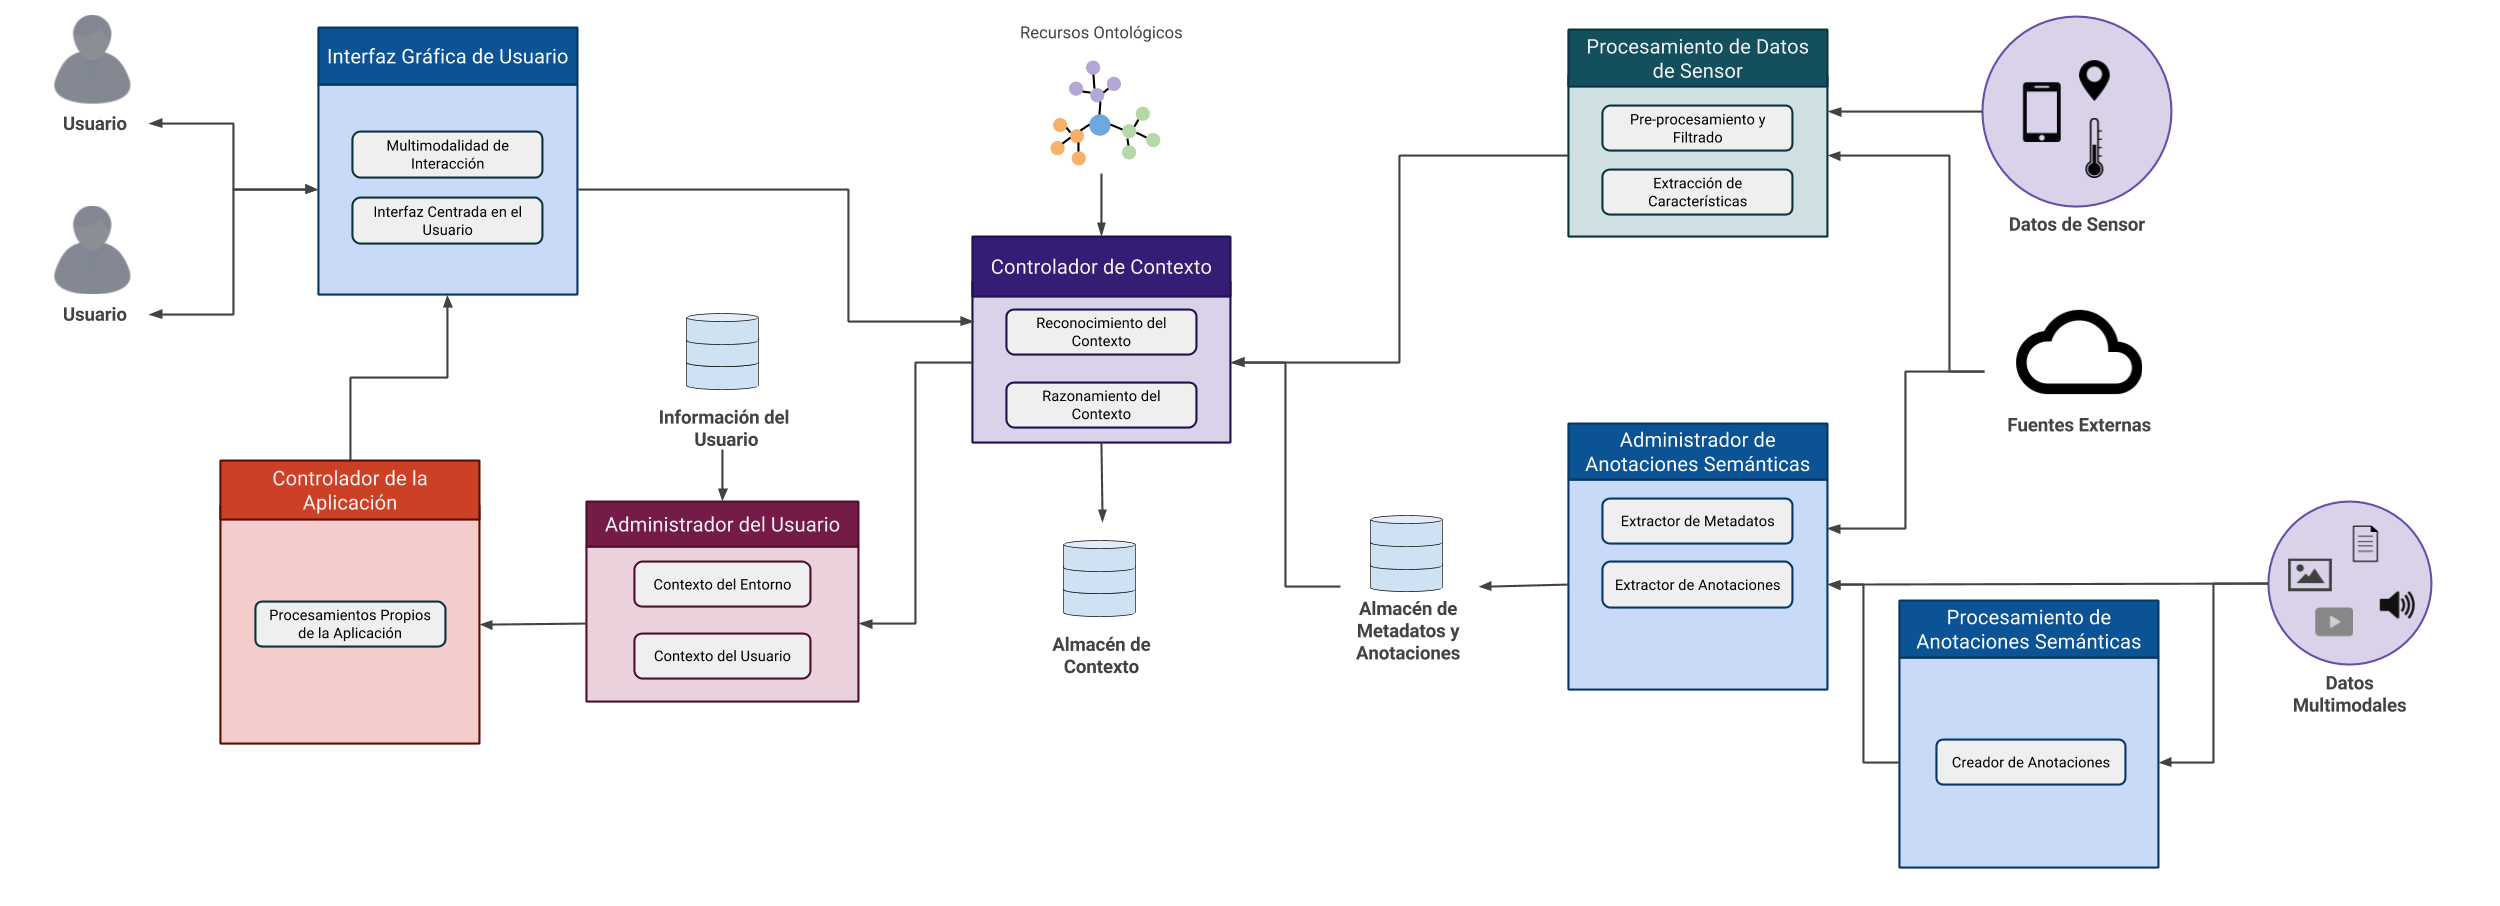
\includegraphics[width=\textwidth]{Cap3/Images/Diagrama_General}%
\caption{Diagrama general del sistema sensible al contexto multimodal.} \label{fig:Diagrama_General}
\end{figure}

% Antes de empezar con la descripción de la arquitectura se deben definir algunos términos: (i) Ítem: Cualquier elemento que pueda ser sugerido al usuario, puede ser un objeto por comprar, un lugar por visitar o una actividad por desarrollar, (ii) etiqueta: es el texto asociado a un contenido multimedia, (iii) anotación: texto que se asocia solo a una parte del contenido \cite{bracamonte2017extracting}. También es necesario definir un lenguaje de marcado que permita la interoperabilidad entre plataformas como XML o RDF \cite{nanarvaez2016modelo, barnaghi2013linked}.

% \begin{enumerate}

% \item Datos Multimodales: Son datos capturados en diferentes formatos por los usuarios, pueden tener algún tipo de relación por localización o por fecha de captura, y se obtienen por medio de un dispositivo de interacción.
% \item Datos de Sensor: Se obtienen a partir de redes de sensores que tienen acceso a internet y que describen las características del entorno de una entidad.
% \item Fuentes externas: Son datos que no son creados por el usuario ni son capturados con dispositivo de interacción, pueden describir el estado de una entidad o proveer información adicional que ayude a obtener el contexto.
% \item Administrador de Datos Multimodales (ADM): Su propósito es obtener la información para la creación de los objetos archivo y multimedia propuestos por Narvaez et al. [15], tiene en cuenta etapas de extracción de metadatos, anotaciones y etiquetas. Para realizar las etiquetas y anotaciones se pueden usar estrategias manuales, semiautomáticas o automáticas. 
% \item Administrador de Datos del Sensor (ADS): Procesa la información obtenida de los sensores eliminando datos atípicos. Adicionalmente, utiliza estrategias de clasificación para identificar automáticamente la acción que desarrolla un usuario. Tanto el ADM como el ADS envía anotaciones textuales que serán analizadas por el Administrador de Contexto.
% \item Almacén de Metadatos y Anotaciones: Dado que obtener las características de los contenidos cada vez que el usuario lo requiera es costoso, cuando se registra un nuevo contenido el ADM lo procesa y los resultados son almacenados en este componente. Mientras que los datos de sensor son analizados en tiempo real, los datos multimodales serán analizados una vez y podrán ser actualizados.
% \item Recursos Ontológicos: Las ontologías son el modelo de representación recomendado en este trabajo. Según Perera et al. [6] las ontologías permiten el intercambio de información entre sistemas y facilitan el proceso de razonamiento sobre las variables de contexto, se recomienda combinar estrategias de razonamiento para hacer el algoritmo mucho más confiable.
% \item Administrador de Contexto: Realiza los llamados al ADM y ADS para obtener las variables de contexto, y realiza procesos de razonamiento logrando que el sistema actúe automáticamente en la recomendación. Las ontologías, son la fuente principal de información para el modelado y razonamiento de contexto en esta propuesta.
% \item Administrador del Usuario: Procesa la información del usuario y el entorno para seleccionar el contexto más adecuado según sus preferencias e historial de actividades desarrolladas.
% \item Información del Usuario: Almacena la información personal del usuario y sus preferencias en ítems y contexto.
% \item Sistema de Recomendación: Obtiene los datos de los ítems que se pueden usar en el proceso de recomendación, como se indicó en la sección 2.3 el tipo de recomendación puede variar dependiendo de la calidad, cantidad y tipo de datos de los que se disponga; y de la aplicación que se va a dar al sistema. Luego los datos se filtran de acuerdo a la información contextual identificada y finalmente se realiza la recomendación.
% \item Contenidos del Dominio: Es la información de los ítems que serán analizados y recomendados por el sistema.
% \item Usuario: Quien desea obtener una recomendación por parte del sistema.


% \end{enumerate}

\subsection{Multimedia Context}
\label{sec:Prop_MultimediaContext}

\section{Contexto}
\label{sec:Prop_Contexto}

En este capítulo se presentan los \textbf{aportes} (son aportes? algunas cosas solo las vamos a usar no mejorar) en los diferentes aspectos del ciclo de vida del contexto presentado por Perera et al. \cite{Perera2014}. En la sección \ref{subsec:Prop_Modelado} se definen los componentes ontológicos con los que se representará el contexto mientras que en las secciones \ref{subsec:Prop_Adquisicion}, \ref{subsec:Prop_TransDatos} \ref{subsec:Prop_Razonamiento} y \ref{subsec:Prop_Servicio} se presentan a detalle los componentes del modelo de la figura \ref{fig:Diagrama_Contexto}, este modelo tiene en cuenta trabajos del estado del arte en razonamiento y modelado del contexto (CITAS) y está compuesta por las siguientes capas: (CÓMO PONERLE QUE EL MODELO ES DEL PROCESO DE CONTEXTO SIN REPETIR TANTO?)

\begin{itemize}
    \item Captura de datos: Capa dedicada a la adquisición de los datos relevantes para el sistema de contexto, tiene en cuenta las entidades que intervienen en la interacción, los contenidos multimedia y los datos obtenidos de fuentes externas. Adicionalmente se encarga de limpiar y organizar la información para su posterior transformación.
    \item Transformación de datos: Transforma la información al formato RDF permitiendo la interoperabilidad con otros sistemas y facilitando el uso de redes semánticas para la descripción del contexto del usuario.
    \item Razonamiento: Analiza los datos capturados para encontrar el contexto que describe las situaciones de un usuario, cuenta con un conjunto de reglas relevantes según cada uno de los usuarios, asegurando la personalización en los servicios a proveer.
    \item Servicio: Presenta al usuario los servicios identificados en la etapa de razonamiento, tiene en cuenta los dispositivos de interacción y los gustos y necesidades del usuario. Este componente se verá afectado por las actividades que el usuario requiere haga el sistema.
\end{itemize}

% \begin{figure}[ht]
% \centering%
% \includegraphics[width=\textwidth]{Cap3/Diagrama_Contexto}%
% \caption{Arquitectura de contexto MCARS.} \label{fig:Diagrama_Contexto}
% \end{figure}

\begin{figure}[ht]
\centering%
\includegraphics[width=\textwidth]{Cap3/Images/Diagrama_Contexto_v2}%
\caption{Arquitectura de contexto MCARS.} \label{fig:Diagrama_Contexto}
\end{figure}


\cite{Avenoglu2017} dice que separar la administración del contexto y las operaciones de adaptación al contexto permite especializar el sistema.

\subsection{Modelado de Contexto}
\label{subsec:Prop_Modelado}

Como se indica en la sección \ref{sec:MT_SensibilidadContexto} las ontologías son la estrategia de modelado de contexto que hemos seleccionado en este trabajo, la decisión se respalda en \textbf{\textit{(i)}}el estado del arte realizado por (CITA SURVEY) \cite{Iaz2014} quien indica que las ontologías son ampliamente usadas para modelar el contexto, \textbf{\textit{(ii)}} trabajos relacionados con Alzheimer y Sensibilidad al contexto (CITAS) que las usan como método de representación, y \textbf{\textit{(iii)}} conocimientos previos en el área por parte de los desarrolladores de este trabajo.

Algunos trabajos han tratado la producción de ontologías de contexto en diferentes áreas del conocimiento \cite{Iaz2014} Iaz et al. presenta un estudio en donde identifica las ontologías de contexto más usadas y las califica de acuerdo a factores cómo la calidad de la representación del entorno del usuario y la facilidad de utilización y reuso. Ontologías de contexto como CONON(2004) y CoBrA(2003) obtienen el cuarto y sexto puesto respectivamente y mIO!(2010) y PiVOn(2010) obtienen los mejores lugares con el noveno y decimo, un factor de gran importancia son las tecnologías y estándares disponibles cuando fueron hechas las propuestas por esta razón es pertinente evaluar las propuestas que modelan el contexto por medio de ontologías en años recientes.

Villalonga et al.\cite{Villalonga2015} propone una ontología de contexto que se centra en las actividades de un usuario y que divide el contexto en bajo (componentes mínimos del contexto) y alto nivel (combinación de varios contextos de bajo nivel), algunas de las clases que componen el contexto de bajo nivel son Emoción,  Lugar y Actividad; mientras que el alto nivel está compuesto por Actividades Físicas como Trabajar en la Oficina o Dormir. En este sistema los datos que ingresan son etiquetas realizadas a datos de sensor y a contenidos multimedia, sin embargo no se hace una representación de los contenidos en el modelado de contexto, las imágenes producto de los vídeos son tomados como salida de un sensor. El modelado de contexto también ha sido trabajado en el ámbito de las casas inteligentes, Men y Lu \cite{Meng2016} proponen una ontología de alto nivel que se centra en el contexto y que representa al usuario, los dispositivos, la red, el entorno, la localización, el tiempo y la historia. En el trabajo indican que los datos binarios hacen parte de una ontología de bajo nivel.(LEER MAS)
Bravo et al.\cite{Bravo2017} propone una ontología que representa el contexto en una entidad educativa y que se divide en tres partes usuario, dispositivo (incluyendo sensores) y entorno. Y Cabrera et al. \cite{Cabrera2017} propone dividir la base de conocimiento en tres partes una ontología de alto nivel que representa las clases principales del contexto el tiempo, el perfil, el entorno, el rol, el estado, la localización, la actividad, los recursos y los agentes; una ontología de mediano nivel que permite usar recursos ontológicos externos como foaf o time ontology y una ontología de bajo nivel que es específica del dominio y extiende la información en el mediano nivel.
En el área de e-health Fissan et al. \cite{Fissaa2017} presenta una ontología desarrollada en OWL-S que se centra en los servicios que puede entregar el sistema y que representa el contexto con las clases usuario, dispositivo, entorno e información médica. En la misma área se ha implementado una ontología basada en las 5Ws (Where....) que incluyen usuario, actividad, tiempo, dispositivo, servicio y localización; en este caso los contenidos de la ontología varian de acuerdo al dominio de la aplicación pero no se manejan dos capas \cite{Aguilar2017}.

\todo{Revisar este párrafo}
Los trabajos de Villalonga et al.\cite{Villalonga2015} y Cabrera et al. \cite{Cabrera2017} presentan ontologías que pueden ser usadas en este trabajo la ontología de 3 niveles de Villalonga es bastante grande y cuenta con información que no es relevante para esta propuesta incluso si se están modelando las mismas clases; en cuanto a la propuesta de dividir la ontología por medio del contexto parece facilitar las actividades de razonamiento que ejecuta la ontología pero igual mente no tiene suficientes conexiones entre las clases del contexto de alto nivel, limitando el razonamiento solo a descubrir información de la actividad y no relaciones que puedan ser pertinentes entre los elementos para llegar a un contexto mejor definido.  %REVISAR ESTE PÁRRAFO

Gracias a los trabajos anteriormente mencionados fue posible identificar las clases más importantes a reflejar en el modelado de contexto el lugar, el tiempo y los usuarios hacen parte de la mayoría de los modelos; aunque en algunos casos el modelado del usuario se limita de definir un identificador del mismo mientras en otros presentan información de su rol en la actividad y sus datos personales. La representación de los dispositivos no se da en todos los trabajos pues en algunos no es importante modelar toda la información de los sensores, depende más del dominio en el cual se aplicará el sistema.
Finalmente variables como las actividades y los servicios se usan en propuestas que desean incluir en la representación la forma como el sistema reaccionará con el cambio del contexto, lo cual no es necesario en todos los dominios.
Se puede ver una diferencia entre lugar y entorno, en las propuestas un lugar tiene características como localización, tamaño y si es cerrado o abierto; mientras que el entorno guarda variables como la temperatura de un lugar o el número de personas que lo ocupan en un momento determinado. Dada esta diferenciación en algunos casos el entorno se modela como una subclase del lugar y en otros son dos clases totalmente diferentes.
En cuanto a la composición de las ontologías estas son divididas en capas buscando facilitar su implementación en diferentes dominios. Aunque en algunas propuestas se indica el uso de una sola ontología, es claro que primero se deben plantear las clases que representan el contexto de forma general y luego se incorpora la nueva información, por lo tanto el uso de capas permite mejorar el proceso de incorporar nuevo conocimiento en la base de información. Teniendo en cuenta que una ontología general permite modelar diferentes eventos pero no es capaz de asistir a usuarios en actividades determinadas y que una ontología específica no permite reutilizar correctamente los recursos modelados \cite{Iaz2014} en este trabajo se usarán ontologías siendo una la capa de alto nivel y la otra la capa del dominio.    

% Finalmente se tiene en cuenta la disponibilidad de las ontologías y se encuentra que solo 2 de las 6 propuestas ponen a disponibilidad las ontologías desarrolladas.

Villalonga et al. \cite{Villalonga2015} indica que es posible usar combinaciones de contenidos multimedia para reconocer las actividades que realiza una entidad lo cual indica la necesidad de incluir multimedia como entidad y no como resultado de un sensor (PORQUÉ PONERLO COMO ENTIDAD Y NO COMO OUTPUT DE UN SENSOR), \cite{Lazarou2016} incluye datos producto de vídeo para la identificación de actividades.

Una tabla con el resumen de la información anteriormente presentada se puede encontrar en la tabla \ref{tbl:Mod_Ontol}


%IMPORT DE LA TABLA

\begin{table}[ht]
  \begin{center}
    \caption{Your first table.}
    \label{tbl:Mod_Ontol}
    \begin{tabular}{l|c|r} % <-- Alignments: 1st column left, 2nd middle and 3rd right, with vertical lines in between
      \textbf{Value 1} & \textbf{Value 2} & \textbf{Value 3}\\
      $\alpha$ & $\beta$ & $\gamma$ \\
      \hline
      1 & 1110.1 & a\\
      2 & 10.1 & b\\
      3 & 23.113231 & c\\
    \end{tabular}
  \end{center}
\end{table}


% \begin{table}[]
% \centering
% \caption{My caption}
% \label{my-label}
% \begin{tabular}{lllllll}
% \hline
% \multicolumn{1}{c}{\textbf{Propuesta}} & \multicolumn{1}{c}{\textbf{Temática}} & \multicolumn{1}{c}{\textbf{Número de Ontologías}} & \multicolumn{1}{c}{\textbf{Clases}}                                           & \multicolumn{1}{c}{\textbf{Centrado en}} & \multicolumn{1}{c}{\textbf{Ontologías Externas}} & \multicolumn{1}{c}{\textbf{Disponible}} \\ \hline
% \cite\{Villalonga2015\}                & General                               & 1                                                 & Usuario, Actividad, Localización, Emoción, Tiempo                             & Usuario Actividades                      & No                                               & Si                                      \\
% \cite\{Meng2016\}                      & Casa Inteligentes                     & 1                                                 & Usuario, Dispositivo, Red, Entorno, Localización, Tiempo, Historia            & Dispositivos                             & No                                               & No                                      \\
% \cite\{Bravo2017\}                     & Escuelas inteligentes                 & 1, dividida en 3 partes.                          & Persona, Dispositivo, Entorno                                                 & Usuario                                  & No                                               & No                                      \\
% \cite\{Cabrera2017\}                   & General                               & 3, Alto, Medio y Bajo nivel                       & Tiempo, Perfíl Entorno, Rol, Estado, Localización, Actividad, Recurso, Agente & Usuario                                  & Si                                               & Si                                      \\
% \cite\{Fissaa2017\}                    & E-Health                              & 1 ontología                                       & Servicio, Usuario, Dispositivo, Entorno, Dominio                              & Servicios                                & Si                                               & No                                      \\
% \cite\{Aguilar2017\}                   & General                               & 1                                                 & Usuario, Actividad, Tiempo, Dispositivo, Servicio, Localización               & Usuario                                  & Si                                               & No                                      \\ \hline
% \end{tabular}
% \end{table}

% Emoción
% Lugar *****
% Actividad (bajo y alto nivel) **
% Usuario(ROL) ****
% Dispositivo ***
% Red *
% Entorno **
% Tiempo ****
% Historia *
% Agentes *
% Servicio *


% \cite{Iaz2014} Equally important is having an adequate level of action granularity (e.g., tasks,
% activities, behaviors, etc.) for a specialized and incremental discovery. A formalized
% and common representation of universal entities, such as time, geographical indoor
% and outdoor locations, and environmental conditions, would greatly help in these pro-cesses.


\subsubsection{Ontología del Contexto - mContext}
\label{subsubsec:Prop_Mod_mContext}

Las clases y relaciones serán representadas en una ontología mediante el lenguaje OWL2 del W3C en la herramienta protégé \footnote{https://protege.stanford.edu} con lo cual se obtiene la ontología de alto nivel pues contiene la estructura general y las clases necesarias para obtener el contexto en diferentes sistemas. Existen muchas formas de modelar una ontología, Noy y McGuinness \cite{noy2001ontology} presentan un proceso de 7 pasos que van desde la definición del dominio de la ontología hasta la identificación de las propiedades entre los elementos de la base de conocimiento, los pasos son
\textbf{\textit{(i)}} determinar el dominio y límite la ontología, 
\textbf{\textit{(iii)}} enumerar los términos relevantes dentro de la ontología,
\textbf{\textit{(ii)}} considerar las ontologías que se pueden reutilizar,
\textbf{\textit{(iv)}} definir la jerarquía de clases,
\textbf{\textit{(v)}} definir las propiedades de las clases,
\textbf{\textit{(vi)}} definir las características de las propiedades identificadas,
\textbf{\textit{(vii)}} poblar la ontología con los individuos necesarios.

Las posiciones de los pasos 2 y 3 han sido modificados de forma voluntaria pues creemos pertinente definir los términos relevantes antes de identificar fuentes de información externas que puedan ser empleadas. A continuación se presentan los resultado de cada una de las etapas para el modelado de la ontología de alto nivel, el desarrollo de la ontología de bajo nivel (Dominio) será tratada en la sección \ref{sec:CS_Ont_Dominio}.

\textbf{\textit{(i) determinar el dominio y límite la ontología}}

En esta etapa se debe responder a las siguientes preguntas 

\begin{itemize}
    \item ¿Cuál es el dominio que cubrirá la ontología? - Esta ontología representará el dominio del contexto computacional y estará centrado en el usuario por lo tanto no se presentará información específica acerca de dispositivos y redes.
    \item ¿Para qué se va a usar la ontología? - La ontología permitirá conectar los componentes del dominio para facilitar las tareas de razonamiento y la adquisición de conocimiento.
    \item ¿A qué tipo de preguntas debería responder la ontología? - esta ontología debería poder responder a preguntas cómo ¿En cuáles lugares estuvo el usuario el día miércoles?, ¿El usuario tenia compañía cuando sucedió esta actividad?, ¿Por cuanto tiempo desarrolló el usuario la actividad?. Serán preguntas relacionadas con el contexto que se ha identificado para el usuario.
    \item ¿Quien usará y mantendrá la ontología? - La ontología será usada por sistemas que deban reflejar el contexto desde un ámbito centrado en los usuarios y que deseen contar con referencias a bases del conocimiento establecidas y soportadas. La ontología se pondrá a disposición de otros usuarios y estos podrán mantenerla de ser necesario.
\end{itemize}

\textbf{\textit{(iii) enumerar los términos relevantes dentro de la ontología}}

\begin{figure}[!ht]
\centering%
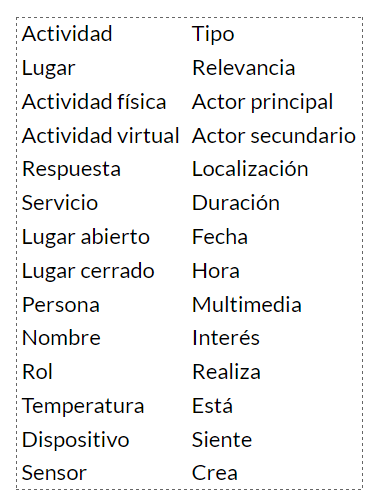
\includegraphics[width=0.3\textwidth]{Cap3/Images/Contexto_Modelado_Terminos}%
\caption{Terminos que relevantes de la ontología.} \label{fig:Contexto_Modelado_Terminos}
\end{figure}

Se realiza una lluvia de ideas teniendo en cuenta las acciones que desarrollan los usuarios de un sistema de contexto en diferentes casos de estudio luego algunas palabras son agrupadas y analizadas de acuerdo al conocimiento en el área. Las palabras resultantes se pueden observar en la figura \ref{fig:Contexto_Modelado_Terminos}


\textbf{\textit{(ii) considerar las ontologías que se pueden reutilizar}}

Luego de identificar los conceptos relevantes para la ontología se identifican los recursos usados en otras propuestas del estado del arte. Teniendo en cuenta que la búsqueda de ontologías en la actualidad no es tarea fácil dada la desactualización de las fuentes y los sistemas de búsqueda, se opta por el uso de fuentes encontradas en el sistema Linked Open Vocabularies (LOV) \footnote{http://lov.okfn.org/dataset/lov/} y propuestas por la W3C. A continuación se presenta la tabla \ref{tbl:Mod_Extern_Ontology} en donde se encuentran las ontologías usadas para ampliar los significados de las clases de la ontología de contexto.

\todo[]{https://www.w3.org/TR/activitystreams-vocabulary/}
Tener en cuenta y % https://www.w3.org/ns/activitystreams

% http://ld-r.org/



%IMPORT DE LA TABLA
\begin{table}[ht]
\centering
\caption{Recursos ontológicos externos}
\label{tbl:Mod_Extern_Ontology}
\begin{tabular}{lll}
\hline
\multicolumn{1}{c}{\textbf{Ontología de Contexto}}                                   & \multicolumn{1}{c}{\textbf{Ontología Externa}}                                              & \multicolumn{1}{c}{\textbf{Ejemplo de Componentes}} \\ \hline
\multicolumn{1}{l|}{Persona}                                                         & \multicolumn{1}{l|}{Foaf \tablefootnote{http://xmlns.com/foaf/spec/}}                                                                   & foaf:Agent, foaf:Person                             \\
% \multicolumn{1}{l|}{Rol}                                                             & \multicolumn{1}{l|}{Foaf \tablefootnote{http://xmlns.com/foaf/spec/}}                                                                   & foaf:Group                                          \\
\multicolumn{1}{l|}{\begin{tabular}[c]{@{}l@{}}Dispositivo\\  y Sensor\end{tabular}} & \multicolumn{1}{l|}{SSN \tablefootnote{https://www.w3.org/TR/vocab-ssn/}}                                                                    & sosa:Sensor, sosa:Observation                       \\
\multicolumn{1}{l|}{Multimedia}                                                      & \multicolumn{1}{l|}{\begin{tabular}[c]{@{}l@{}}OMR \tablefootnote{https://www.w3.org/ns/ma-ont}\\ M3 - adaptación\\ Dolce?\end{tabular}} & ma:MediaResource                                    \\
\multicolumn{1}{l|}{Lugar}                                                           & \multicolumn{1}{l|}{\begin{tabular}[c]{@{}l@{}}GeoNames \tablefootnote{http://www.geonames.org/ontology/documentation.html}\end{tabular}}              & geo:lat, geo:long, genames:nearby                   \\
\multicolumn{1}{l|}{Tiempo}                                                          & \multicolumn{1}{l|}{Time Ontology \tablefootnote{https://www.w3.org/TR/owl-time/}}                                                          & time:dayOfWeek, time:TemporalEntity                    \\ \hline
\end{tabular}
\end{table}


% \begin{table}[h!]
% \centering
% \caption{Recursos ontológicos externos}
% \label{tbl:Mod_Extern_Ontology}
% \begin{tabular}{lll}
% \hline
% \multicolumn{1}{c}{\textbf{Ontología de Contexto}}                                   & \multicolumn{1}{c}{\textbf{Ontología Externa}}                                              & \multicolumn{1}{c}{\textbf{Ejemplo de Componentes}} \\ \hline
% \multicolumn{1}{l|}{Persona}                                                         & \multicolumn{1}{l|}{Foaf \tablefootnote{http://xmlns.com/foaf/spec/}}                                                                   & foaf:Agent, foaf:Person                             \\
% \multicolumn{1}{l|}{\begin{tabular}[c]{@{}l@{}}Dispositivo\\  y Sensor\end{tabular}} & \multicolumn{1}{l|}{SSN \tablefootnote{https://www.w3.org/TR/vocab-ssn/}}                                                                    & sosa:Sensor, sosa:Observation                       \\
% \multicolumn{1}{l|}{Multimedia}                                                      & \multicolumn{1}{l|}{\begin{tabular}[c]{@{}l@{}}OMR \tablefootnote{https://www.w3.org/ns/ma-ont}\\ M3 - adaptación\\ Dolce?\end{tabular}} & ma:MediaResource                                    \\
% \multicolumn{1}{l|}{Lugar}                                                           & \multicolumn{1}{l|}{\begin{tabular}[c]{@{}l@{}}GeoNames \tablefootnote{http://www.geonames.org/ontology/documentation.html}\\ Schema \tablefootnote{http://schema.org/Place}\end{tabular}}              & geo:lat, geo:long, genames:nearby                   \\
% \multicolumn{1}{l|}{Tiempo}                                                          & \multicolumn{1}{l|}{Time Ontology \tablefootnote{https://www.w3.org/TR/owl-time/}}                                                          & time:dayOfWeek, time:hasDuration                    \\ \hline
% \end{tabular}
% \end{table}



% foaf = http://xmlns.com/foaf/spec/
% ssn =  https://www.w3.org/TR/vocab-ssn/
% time = https://www.w3.org/TR/owl-time/#time:dayOfWeek
% multimedia=  https://www.w3.org/ns/ma-ont
% location = http://www.geonames.org/ontology/documentation.html - http://schema.org/Place
\todo{Meter en la tabla Rol con foaf (no estoy seguro)}

% foaf = http://xmlns.com/foaf/spec/
% ssn =  https://www.w3.org/TR/vocab-ssn/
% time = https://www.w3.org/TR/owl-time/#time:dayOfWeek
% multimedia=  https://www.w3.org/ns/ma-ont
% location = http://www.geonames.org/ontology/documentation.html - http://schema.org/Place

\todo{Definir si la ontología con extensiones hace parte del dominio o de la upper}
\textit{\textbf{Esta ampliación hace parte de la ontología del dominio?}}\\


\textbf{\textit{(iv) definir la jerarquía de clases}}

Partiendo de los términos relevantes identificados en el paso (iii) de la metodología y siguiendo los indicios de las clases encontradas en el estado del arte se opta por modelar el contexto usando los siguientes conceptos \textbf{\textit{Persona, Rol, Actividad, Lugar, Sensor, Dispositivo, Servicio, Tiempo y Multimedia}}. Los términos que no se convierten en clases fueron analizados y seleccionados para convertirse en propiedades que describen o relacionan las entidades de la ontología.

\todo{Actualizar la jerarquía poniendo con objeto}
En la figura \ref{fig:Contexto_Modelado_Jerarquia} se presenta la jerarquía de la ontología de alto nivel. Dado que la ontología del dominio depende del caso de estudio esta se presenta con mayor detalle en la sección \ref{sec:CS_Ont_Dominio} en esta solo se mostrará la relación entre las nuevas clases incluidas.

\begin{figure}[!hb]
\centering%
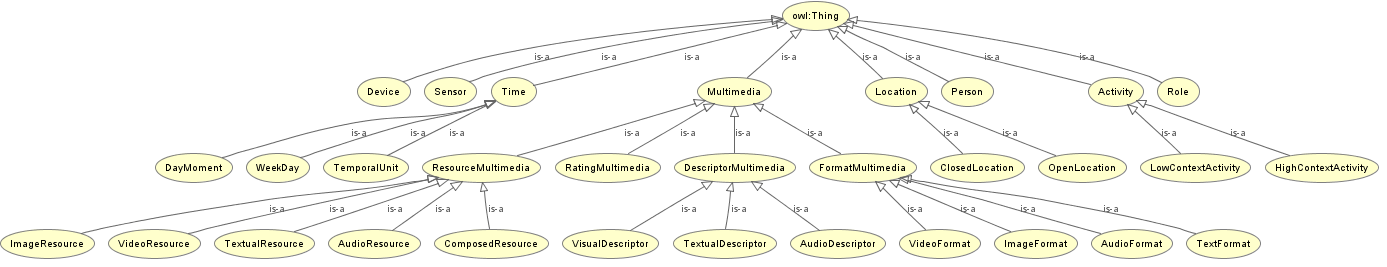
\includegraphics[width=\textwidth]{Cap3/Images/Contexto_Modelado_Jerarquia}%
\caption{Jerarquía de las clases de la ontología.} \label{fig:Contexto_Modelado_Jerarquia}
\end{figure}


\textbf{\textit{(v, vi) definir las propiedades de las clases y sus características}}

En esta etapa se identifican las propiedades de la ontología, se entienden propiedades como valores que describen entidades y relaciones existentes entre las entidades. En el diagrama \ref{fig:Contexto_Modelado_Relaciones} se puede ver la interacción entre las clases principales de la ontología por ejemplo un contenido multimedia describe una actividad y un dispositivo o una persona pueden crear contenidos multimedia.

\todo{Actualizar a nueva versión con objeto, poner versión de protégé?}
\begin{figure}[ht]
\centering%
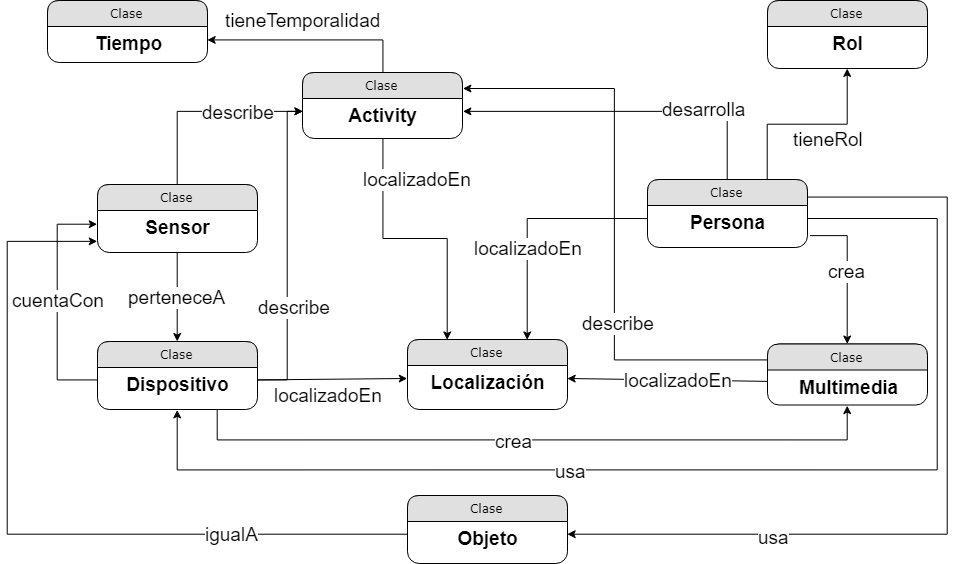
\includegraphics[width=0.8\textwidth]{Cap3/Images/Contexto_Modelado_Relaciones}%
\caption{Relaciones principales entre las clases de la ontología de contexto.} \label{fig:Contexto_Modelado_Relaciones}
\end{figure}

De otro lado en la figura \ref{fig:Contexto_Modelado_TipoDato} se presenta una pequeña parte de los valores que describen las clases y las características de estos valores. Por ejemplo la entidad persona tiene la propiedad nombre que es del tipo de dato Literal.

\begin{figure}[ht]
\centering%
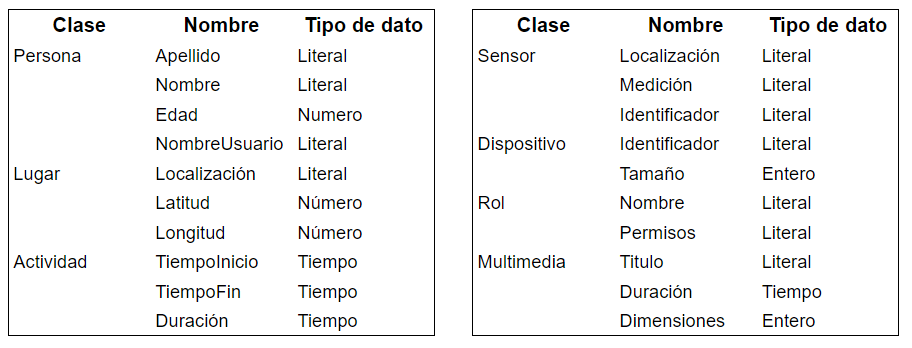
\includegraphics[width=0.9\textwidth]{Cap3/Images/Contexto_Modelado_Caract_Relaciones}%
\caption{Características de las propiedades de la ontología.} \label{fig:Contexto_Modelado_TipoDato}
\end{figure}



\textbf{\textit{(vii) poblar la ontología con los individuos necesarios}}

Esta etapa se desarrollará en la sección \ref{sec:CS_Ont_Dominio} cuando se desarrollen los componentes propios del dominio de la aplicación.


% En la figura \ref{Contexto_Upper_Ontology} se puede ver un extracto de la ontología de alto nivel con componentes de ontologías externas.


EN LA PÁGINA \textbf{http://www.visualdataweb.de/webvowl/#iri=http://purl.org/m-context/ontologies/mContext} SE PUEDE VER LA ONTOLOGÍA 

\subsection{Adquisición de Contexto}
\label{subsec:Prop_Adquisicion}

En esta capa se obtienen los datos que serán analizados para encontrar el contexto de la entidad más importante de la propuesta, el usuario. Según Perera et al.\cite{Perera2014} un componente de adquisición debe tener en cuenta aspectos como la frecuencia de obtención y tipo de sensor, en esta arquitectura \textbf{\textit{(i)}} los datos de contexto se obtienen de forma periódica y \textbf{\textit{(ii)}} las fuentes de contexto son variadas. Las fuentes de información de esta propuesta se dividen en 3 grupos:
\begin{itemize}
    \item \textbf{Sensores de Entidades}: Esta categoría sigue la definición de entidad de Dey et al.\cite{Dey2001}, esto es de gran importancia teniendo en cuenta que en la actualidad un auto, una casa, un teléfono o una persona pueden llevar sensores que generan información acerca de su condición y la de su entorno. Es posible entonces combinar información contextual de un vehículo y su conductor (CITA TRABAJO CONTEXTO/RAZONAMIENTO) o de un anciano con su hogar (CITA CONTEXTO/APLICACIÓN).
    \item \textbf{Contenido Multimedia}: Representa el aporte de este trabajo y sigue los lineamientos presentados en las secciones \ref{sec:MT_ContenidosMultimedia} y \ref{sec:Prop_MultimediaContext}. Parte de la hipótesis de que los contenidos que producen los usuarios en diferentes situaciones almacenan información contextual de utilidad para definir las situaciones de una persona en diferentes momentos. Información de contexto de naturaleza social como las personas con las que se compartió un momento, o dependiente de un campo de aplicación en específico como los cantos de algunas aves cuando se realizaba una exploración en campo permiten que una aplicación modifique su funcionamiento y facilite las actividades que este debe realizar.
    \item \textbf{Datos Externos}: Este grupo corresponde a la descripción de Sensores Lógicos presentados por \cite{Perera2014}, con este grupo se asegura el uso de información proveniente de servicios web que puede modificar o complementar el contexto de un usuario. Un ejemplo es el registro del clima en el lugar de interés de un turista, o el listado de eventos sociales que se desarrollan un fin de semana (incluyendo costos y horarios).
\end{itemize}

\subsection{Pre-procesamiento de los datos}
\label{subsubsec:Prop_Adqui_PrePro}

De acuerdo al ciclo de vida de los sistemas sensibles al contexto es necesario realizar procesos de filtrado de información, este proceso asegura la eliminación de datos fuera de orden, la unión de mediciones ocurridas en periodos iguales de tiempo y también la identificación del contexto de bajo nivel por medio de la identificación de actividades de forma automática.
El pre-procesamiento de los datos dependerá de las tecnologías pertinentes al sistema al desarrollar, en este trabajo se propone una arquitectura de tres capas con las siguientes características, Fig  \ref{fig:Diagrama_preprocesa}:
\textbf{\textit{(i)}} fuentes de contexto, 
\textbf{\textit{(ii)}} tipos de dato producidos por las fuentes de contexto,
\textbf{\textit{(iii)}} algoritmos de procesamiento,
\textbf{\textit{(iv)}} uso de estándares para el etiquetado de actividades reconocidas.
\begin{figure}[ht]
    \centering%
    \includegraphics[width=\textwidth]{https://docs.google.com/drawings/d/1pNA08-j5f8h--PJIRJZafjfwxJ1rQbj0zHwOFvc57LA/edit     Cap3/Images/Diagrama_Contexto_v2}%
    \caption{Arquitectura de contexto MCARS.} \label{fig:Diagrama_preprocesa}
\end{figure}
    


sigue los parámetros presentados en la Arquitectura General \ref{sec:Prop_Arquitectura} (O CITAR EL COMPONENTE DE LA ARQUITECTURA GENERAL).

\subsection{Transformación de datos}
\label{subsec:Prop_TransDatos}

Como se indica en la sección \ref{sec:MT_LinkedData} el uso de datos enlazados permite ....., adicionalmente en esta propuesta facilita el uso de fuentes de información que no se relacionan directamente con el dominio de la aplicación pero que pueden ser de utilidad para definir el contexto del usuario. El propósito principal de esta capa es transformar los datos binarios ( metadatos y etiquetas) a un formato estándar, como RDF, que facilite la interoperabilidad con otros sistemas que hacen uso de bases de conocimiento y la realización de consultas sobre estas. Al finalizar el proceso los datos estarán representados en RDF por lo cual será posible aplicar estrategias de razonamiento sobre ontologías que clasifiquen e identifiquen rápidamente el conjunto de reglas que se pueden operar.

\todo{Esto necesita una cita!}
El modelo principal de información para llevar a cabo esta transformación es la ontología mContext presentada en la sección \ref{subsubsec:Prop_Mod_mContext} y los datos a transformar son los especificados en la sección \ref{subsubsec:Prop_Adqui_Datos}. Los métodos para realizar esta actividad se basan en el estándar R2RML\footnote{Recomendación W3C: http://www.w3.org/TR/r2rml/} el cual permite transformar contenidos de bases de datos al formato RDF, esto se hace encontrando la relación entre los campos de la base de datos, y las clases y propiedades que tiene una ontología. La necesidad de transformar datos que tienen formatos y orígenes diferentes a los de las bases de datos, como los resultados del llamado a un servició onlíne, han llevado al desarrollo de herramientas como RML \footnote{http://rml.io} el cual permite usar formatos JSON, CSV, ... como origen y luego transformar a RDF teniendo en cuenta los recursos ontológicos que el usuario haya desarrollado o que estén disponibles en la red.





% El uso de datos enlazados en los sistemas sensibles al contexto no ha sido explorado por muchos autores, entre los trabajos realizados se encuentra *****, estos trabajos concluyen *****. La aplicación del paradigma de datos enlazados es una parte importante del desarrollo de este trabajo de investigación pues ----. El proceso general de transformación de datos se puede encontrar a continuación.

\subsubsection{Proceso de Linked Data}
\label{subsubsec:Prop_TransData_LD}
ES NECESARIO DEFINIR ESTO ENTRE ESTA Y LA SIGUIENTE SEMANA

\subsection{Razonamiento de Contexto}
\label{subsec:Prop_Razonamiento}


\subsubsection{MODIFICACIÓN}

CAMBIARÁ RADICALMENTE

Se propone el uso de SPARQL como en el artículo \cite{Meditskos2013, Meditskos2016}
Hay una nueva versión pero aún no está soportada.


Drools para filtrar las posibilidades y no sobrecargar la ontología, reglas ontológicas para actuar directamente sobre el dominio (actividades que se pueden seleccionar) \textbf{CITAS DE QUE ES NECESARIO DISMINUIR LA CARGA EN EL RAZONADOR} \cite{Ordonez2016}, \cite{Hille} - parece que el ontológico es mejor pero no hablan de si desempeño.

proceso 

reglas generales (Drools) --- - -- reglas dom (SWRL)

Esta capa se permite identificar las acciones más relevantes para el usuario a partir de dos componentes de gran importancia una ontología de alto nivel y una base de datos que contiene ontologías y reglas para cada dominio. El uso de ontologías de alto nivel permite disminuir de la carga de procesamiento del razonador y la independencia de la información que se está manejando (división de la información), trabajos como (PONER TRABAJO) usan dos o más ontologías para representar el conocimiento. En este trabajo se propone el uso de dos sistemas de reglas lógicas (i) las reglas de tipo 1 (RT1) \textbf{SWRL} (PONER REFERENCIA AL ESTANDAR) que actuarán sobre las clases y relaciones existentes en la ontología para definir el contexto del usuario, y (ii) las reglas de tipo 2 (RT2) \textbf{Drools (RT2)} con las que es posible modificar el comportamiento de los servicios dependiendo de los atributos encontrados en el contexto. Gracias a la división de las reglas se puede omitir el modelado de los servicios dentro de la ontología de contexto pues las reglas de tipo SWRL actuan solo sobre componentes de la ontología.

El proceso de selección de condiciones se conforma de seis etapas: 

\begin{enumerate}
    \item Filtrado de acciones no relevantes: a partir de la información resultante del razonamiento en la ontología se eliminan las reglas RT1 con lo que se disminuye la cantidad de opciones que deben ser verificadas.
    \item Revisión de las reglas del dominio: se comprueban las RT1 restantes y se obtienen los atributos de contexto identificados, estos atributos de contexto normalmente representan actividades de alto nivel. 
    \item Selección de reglas: a partir de los datos de contexto se evalúan RT2 obteniendo todos los posibles servicios de respuesta del sistema.
    \item Organización de reglas: dado que se pueden obtener uno o mas servicios, estos se organizan de acuerdo al valor de preferencia para el usuario \textbf{(ESPECIFICAR CUALES)}.
    \item Creación del servicio: se envía el servicio a la distribución del contexto en donde se aplicarán las acciones a las entidades de contexto del sistema.
    \item Actualización de reglas: después de que el usuario ha interactuado con el dispositivo se actualizan las reglas y los valores de preferencia de estas.
\end{enumerate}

Se espera que cada uno de los dominios en los que puede actuar la aplicación esté modelado en una ontología y tenga sus propias reglas.
A continuación por medio de



% http://www.miningminds.re.kr/lifelog/context/context-v2.5.owl

Algunas ontologías de contexto son presentadas por
\cite{Bikakis2007}Sirve porque presenta una lista de ontologías de contexto que posiblemente ya no se encuentren habilitadas, dice también los diferentes tipos de razonamiento que existen

% Tengo dos pares que combinan linked data, cada par es de los mismos autores en el mismo año


% http://linkdata.org/ - POSIBLE HERRAMIENTA



% El razonamiento es -----, las formas comunes de razonamiento son : \cite{Bikakis2007}


% La mayoría encontrada usa ontológico y reglas DL (poner todos los artículos que lo hacen), lo anterior obedece a la falicidad de creación de las reglas pero, trabajos como BLA BLA los dos que hablan de métodos aparte señalan el problema del manejo de la incertidumbre que es cuando no se encuentra nada que siga las reglas.



\cite{Garcia-Sola2014} García propone un sistema de razonamiento distribuido que busca mejorar el desempeño de los razonadores ontológicos tomando pequeños fragmentos de la ontología y combinando diferentes métodos de razonamiento como reglas y representación de acciones en arboles.Aunque la propuesta es clara las tecnologías no son específicadas e indica que el cálculo de tiempo para seleccionar los diferentes métodos de razonamiento no es muy certero.

\cite{Avenoglu2017} Presenta un sistema sensible al contexto SOMNIUM que modela las actividades diarias del usuario como un flujo y utiliza reglas del tipo Drools. La información de contexto se usa solo cuando es pertinente dentro del flujo, disminuyendo \textbf{el peso} del procesamiento y recomendando acciones a los usuarios en tiempo real y de acuerdo su rutina. El esquema de la propuesta principal se divide en un componente que ejecuta y administra las actividades del usuario, un componente que ejecuta las reglas y dos componentes que permiten especializar el sistema de acuerdo al dominio en el que se va a ejecutar.



\cite{Iaz2014} 
having hybrid methods with a first data-driven preprocessing stage appears to be the right direction
to benefit from both data- and knowledge-driven computing paradigms.


% \cite{Li2017} Exploran el concepto de los sistemas sensibles al contexto en los submarinos robóticos, específicamente presenta una arquitectura para el razonamiento en sistemas de contexto que utiliza el razonamiento basado en ontologías, en reglas y en redes bayesianas. En esta propuesta se usa una ontología general, una que contiene datos del dominio y otra que se concentra en las aplicaciones o servicios que se pueden desarrollar. Este trabajo es bastante completo en la definición de la estratégia de razonamiento pues por medio del uso de las redes bayesianas logra eliminar la incertidumbre en el sistema de contexto cuando no hay información suficiente. 




% % https://github.com/ubiquitous-computing-lab/Mining-Minds/tree/master/information-curation-layer

% % https://jena.apache.org/getting_started/index.html


% El trabajo de Gu en el año 2004 mostraba un esfuerzo interesante por resolver problemáticas de los sistemas sensibles al contexto como la consistencia y el tiempo de razonamiento de las ontologías. En su propuesta, se presenta una arquitectura de tres capas (aplicación, razonamiento y adquisición de datos) y la ontología de contexto de alto nivel SOCAM que representa las entidades más importantes en los sistemas de contexto. El razonamiento de esta propuesta se da por medio de Logic Reasoning e inference rules \cite{Gu2004}.


% \cite{Chang2017} Presenta un modelo de contexto que tiene en cuenta datos de sensores variados con múltiples entidades como usuario, vehículo y carretera. Realiza el modelado de contexto por medio de ontologías y el razonamiento lo hace de la misma forma, solo que divide este proceso en 2 1 que permite encontrar la situación y otro (que entiendo no es razonamiento sino el uso de actividades guardadas en bases de datos) toma la decisión en el sistema de esta forma evita sobrecargar el mismo, también presenta datos de los tiempos que se demora el sistema en dar respuesta. El problema de este artículo es que no usa contenido multimedia, tampoco lo necesita, aunque tener información de música, texto y otras cosas puede facilitar la toma de decisiones (por ejemplo el uso del móvil en el proceso de conducción), también puede ser muy útil ver los procesos de interacción como multimedia.


% \cite{Razzaq2017} Este trabajo presenta el un componente de contexto para el framework Mining Minds el cual combina el uso de razonamiento con ontologías y MAchine Learning para obtener el contexto, lo anterior porque usar solo el razonamiento es bastante pesado. (no queda tan claro cómo usa la ontología ni tampoco cómo es el proceso de ML ya que es bastante general). Explica el uso de tecnologías cómo SPARQL, adicionalmente presenta una ontología que divide el contexto de alto y bajo nivel (puede servir de guia para el desarrollo de otras ontologías)  
% \cite{Wei2013} presenta una arquitectura para sistemas sensibles al contexto que adapta automáticamente las actividades que se presentan al usuario. Esta arquitectura usa ontologías y para el razonamiento Description Logic y First order logic reasoning. Para la toma de decisiones usa un proceso de filtrado en donde se eliminan primero las tasklets ménos importantes para el contexto y luego dependiendo de lo que sucede en el entorno se evaluan las opciones más optimas. esta propuesta no tiene encuenta los formatos y realiza razonamiento solo con las reglas de las ontologías




% Adaptaciòn automàtica de las decisiones en un sistema sensible al contexto 3 capas - programación (estruct y leng prog), conocimiento (ontolo) y decisión

% Technol
% Composital adaptation
% Ontology
% Description logic/first-order logic reasoning.
% Pellet for description logic
% jess for first-order logic reasoning

% Ontologías
% * Contexto - modela entidades de contexto para compartir información de entornos dinámicos
% * Tareas - taras de un individuo y requerimientos para condiciones contextuales
% * Servicios - propiedades de los servicios sensibles al contexto y los requerimientos para las tareas.

% Decisiones
% Multistage normative decision model (algo como arbol) para elegir las diferentes alternativas para la selección de la tarea. Primero se filtra, luego
% Description logic/first-order logic

% Presenta buenas gráficas de performance


% \cite{Wang}Presenta la creación de una ontología de contexto a partir de la caracterización de entidades como localización, usuario, actividad y computador. Dentro de esta propuesta se presenta también un ejemplo dónde se puede evidenciar el uso de reglas de razonamiento para encontrar contexto a partir de datos de entrada. (leer bien)  

Dadas las problematicas encontradas en el uso de SWRL entre las cuales se encuentra
\textbf{\textit{(i)}} tiempos largos de ejecución del paquete de reglas.
\textbf{\textit{(ii)}} falta de una característica que permita generar instancias en la ontología de forma automática.
Es claro que estas desventajas pueden darse debido al proceso generado para la ejecución de reglas en dos fragmentos.

\subsection{Ontología de Reglas}
\label{subsec:Prop_Razonamiento_Rules_Ont}

\begin{figure}[!ht]
    \centering%
    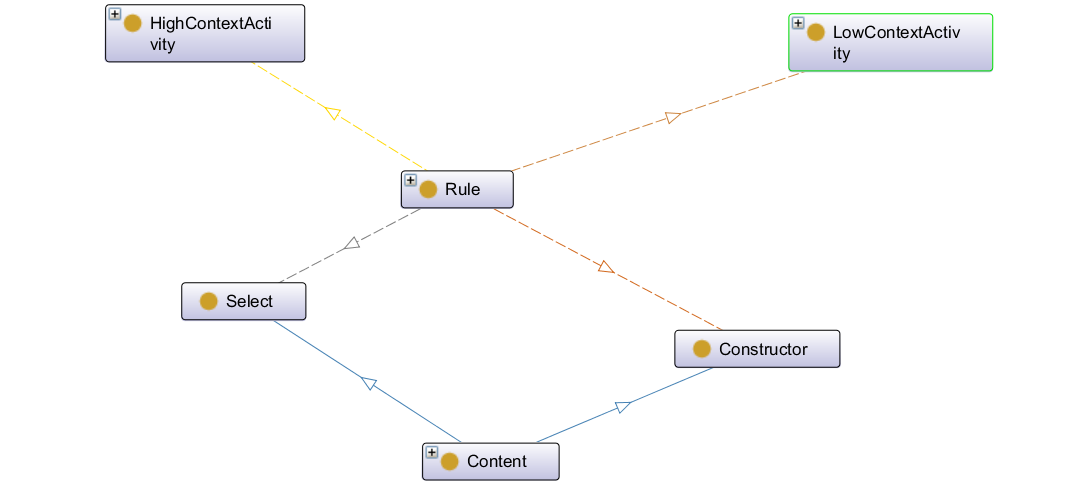
\includegraphics[width=0.3\textwidth]{Cap3/Images/Contexto_Razonamiento_Ont_Rules}%
    \caption{Ontología de Reglas.} \label{fig:Contexto_Razonamiento_Ont_Rules}
\end{figure}

Se crea una ontología, \ref{fig:Contexto_Razonamiento_Ont_Rules} que busca relacionar las actividades de contexto de alto y bajo nivel, presentadas en la ontología de la sección \ref{subsubsec:Prop_Mod_mContext}, con las reglas del dominio.

\subsection{Reglas SPARQL}
\label{subsec:Prop_Razonamiento_SPARQL}

Teniendo en cuenta el rendimiento ofrecido por las reglas SWRL se opta por una alternativa con SPARQL. En la figura \ref{fig:Flujo_reglas_sparql} se puede observar el flujo de aplicación de reglas el cual sigue los siguientes pasos:

\begin{itemize}
    \item 1) Se obtienen las actividades generadas en a un rango específico de tiempo, pueden ser las actividades de un día o las actividades de una hora determinada.
    \item 2) Se busca en el grafo de reglas aquellas instancias que tienen una relación con las actividades por medio de la propiedad isTrigger de la ontología de reglas \ref{subsec:Prop_Razonamiento_Rules_Ont}.
    \item 3) Se extraen los comandos construct y select que conformarán los queries SPARQL a ejecutar en el siguiente paso.
    \item 4) Se ejecutan las reglas y se generan las instancias y propiedades pertinentes.
\end{itemize}

Esta propuesta trata aspectos que no son mencionados por \cite{Meditskos2013} como:
\textbf{\textit{(i)}} manejo de un gran número de reglas en la bd de grafos - en el trabajo no es claro como se realiza la ejecución de cada una de las reglas en el sistema, si se ejecutan todas las posibles o se realiza algún tipo de filtrado.
\textbf{\textit{(ii)}} representación de las reglas en un grafo para la recuperación eficiente de acuerdo a diferentes elementos de la ontología del dominio.
\textbf{\textit{(iii)}} es posible agregar mas componentes a las reglas como lugar o acompañante.

\todo{TABLA DE COMPARACIÓN ENTRE EL USO DE REGLAS CON SWRL Y SPARQL}

\subsection{Servicio}
\label{subsec:Prop_Servicio}

La capa de servicio es la más variable de todas y se encarga de la etapa de distribución del contexto \cite{Perera2014}, dependiendo del dominio de la aplicación puede tener diferentes componentes. En esta arquitectura se proponen dos componentes para esta capa la de actividades del dominio en el que se definen las estrategias que debe seguir cada sistema para entregar los servicios, y el de entrega de servicios en dónde las modificaciones son enviadas a los dispositivos pertinentes. Finalmente, los usuarios por medio de la interacción con los dispositivos experimentan el servicio de contexto.
\chapter{Caso de estudio}
\label{chp:CS}
% ---- problemas del movil
% https://www.unforgettable.org/blog/dementia-calling-phones-for-people-with-dementia/

Para este proyecto la selección de un caso de estudio que permita validar el problema de investigación planteado en el capítulo \ref{sec:Problema} es de vital importancia. Primero se realiza la búsqueda de artículos científicos que relacionan las áreas de comunicación aumentativa y alternativa (CAA), terapia ocupacional, turismo, música, tráfico y educación con los Sistemas Sensibles al Contexto, temáticas como biología/control de plagas, nutrición y noticias fueron descartadas dado que hay pocos trabajos disponibles en el estado del arte o los trabajos se orientan demasiado a la temática de los Sistemas de Recomendación Sensibles al contexto. El análisis permitió seleccionar el problema de los adultos mayores con Alzheimer como el caso de estudio, en la sección \ref{sec:CS_Comparacion} se presenta detalladamente el proceso desarrollado.\\

En la sección \ref{sec:CS_PersonasyAlz} se muestran las características de las personas con Alzheimer, luego el apartado \ref{sec:CS_Aplicaciones} se habla de los desarrollos comerciales y los trabajos de investigación relacionados, en la sección \ref{sec:Escenarios_estudio} se proponen tres casos de estudio y se desarrollan teniendo en cuenta la arquitectura presentada en el capítulo \ref{chp:Propuesta}.


cuales son los datos de contexto que incluye (clases o entidades que representa usuario, carretera, enfermedad), cómo se adquieren (dispositivos), Cuales son las entidades que me permiten representar las situaciones de mi negocio?
Me parece bueno usar algo como lo que hace \cite{Chang2017}



\section{Áreas de Aplicación para el Caso de Estudio}
\label{sec:CS_Comparacion}

Para la identificación del área de aplicación se realiza una búsqueda de los artículos indexados en Scopus, la tabla \ref{tbl:Comp_Area} presenta un resumen de los componentes encontrados en esta exploración y a continuación se presentan brevemente las características de cada área.\\



\begin{figure}[ht]
\centering%
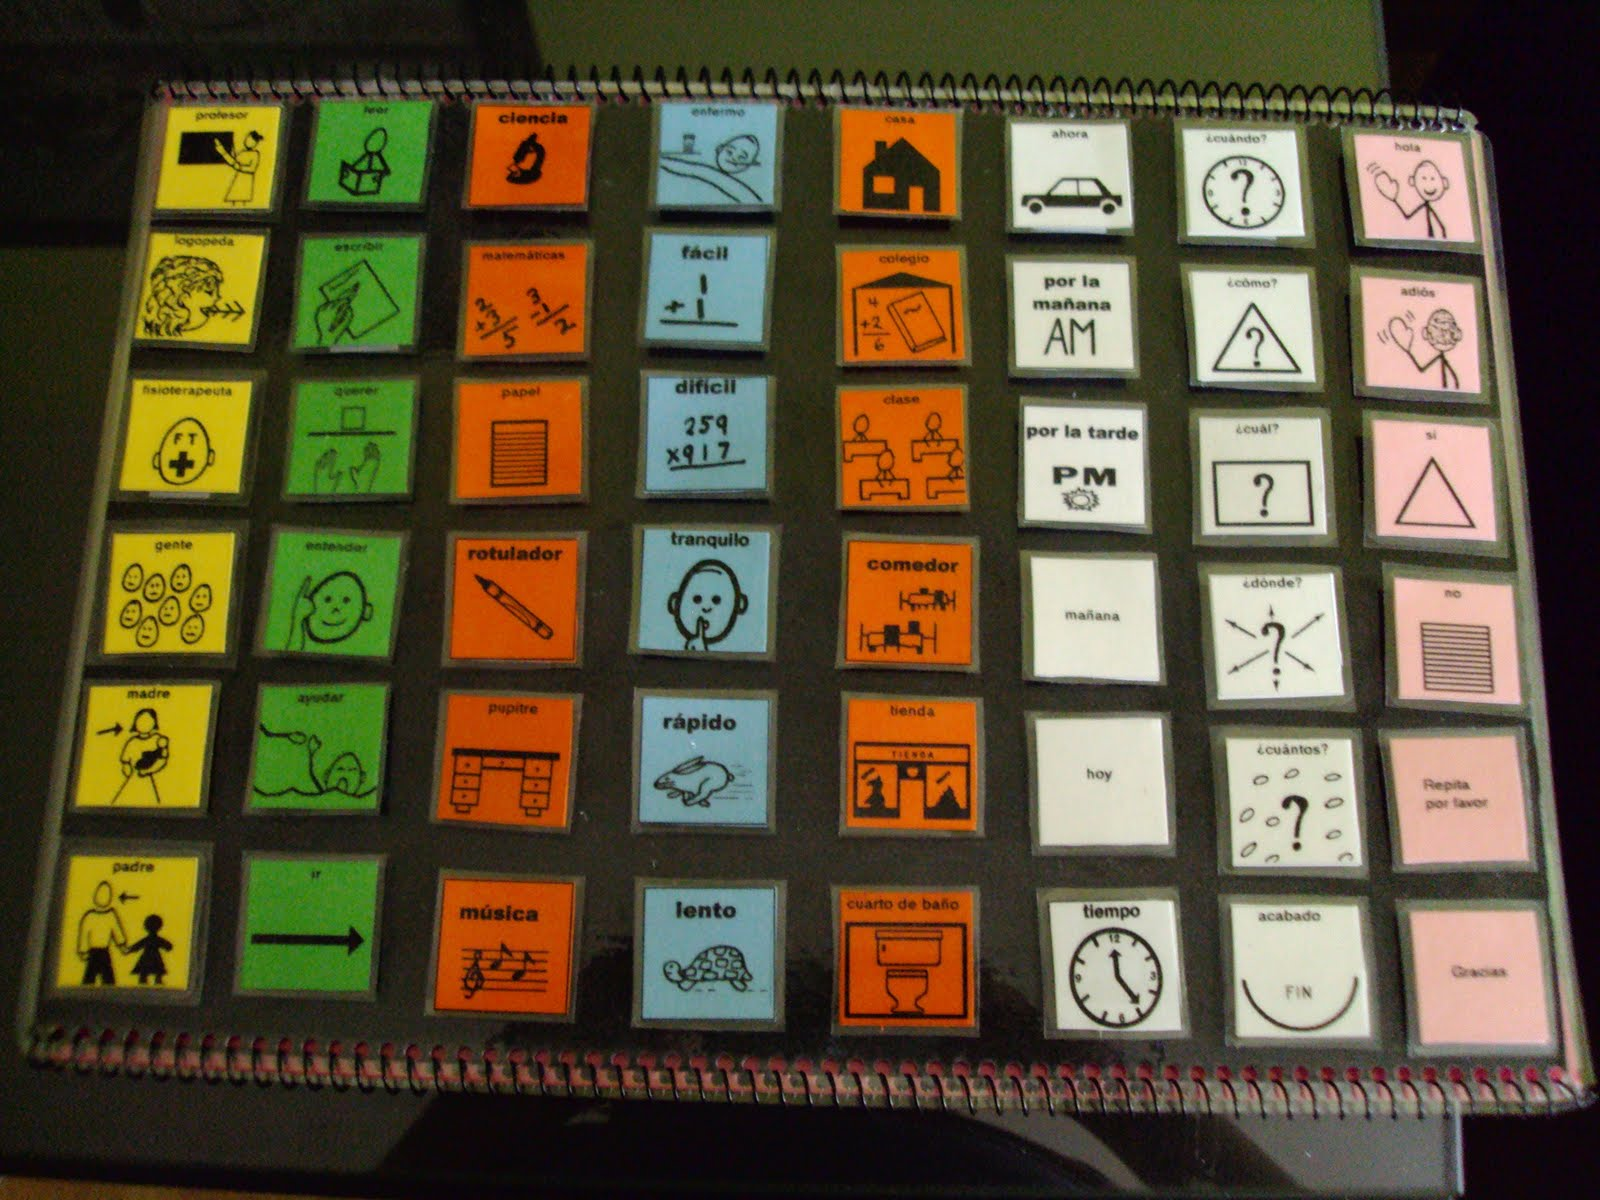
\includegraphics[width=.5\textwidth]{Cap4/tablero_convencional}%
\caption{Diagrama del Razonamiento del sistema.} \label{fig:CAA}
\end{figure}


\textbf{\textit{Comunicación Aumentativa y Alternativa (CAA)}} Los Sistemas CAA buscan formas alternativas de comunicación al lenguaje oral y escrito por medio del uso de tablas de comunicación que pueden ser digitales o análogas. La mayoría de las propuestas en esta área buscan que el usuario pueda generar frases de acuerdo al contexto que están viviendo en el momento logrando que el usuario vea solo contenidos pertinentes y que el tiempo de producción de frases disminuya. Dado que este tipo de sistemas presentan imágenes y textos, ver figura \ref{fig:CAA} estos son los contenidos multimedia que normalmente se emplean, mientras que datos provenientes de sensores como la localización, información del sistema como fecha y hora, e información del usuario como sus preferencias; son las variables contextuales de preferencia.
Resalta en esta área que al parecer no se presenta una forma de representación de conocimiento compleja, en muchos de los trabajos se realizan vínculos por medio de bases de datos de forma jerárquica por esta razón las fuentes de información son propias.\\

\textbf{\textit{Terapia Ocupacional}} En el área de terapia ocupacional se encuentran proyectos que tienen como objetivo hacer seguimiento de las actividades que desarrollan pacientes con enfermedades físicas o mentales, con este seguimiento es posible saber si un paciente ha tomado sus medicamentos, si ha desarrollado las actividades físicas recomendadas, o si se encuentra en situación de peligro. Las interfaces gráficas de estos sistemas están compuestas por imágenes, textos y vídeos que le indican al usuario las acciones que debe realizar, los usuarios normalmente no generan contenidos pero los datos que se obtienen de sensores y la información del usuario (progreso de la enfermedad etc.) son fuente principal de información para la toma de decisiones. En las propuestas encontradas no se utilizan formas de anotación de información ni se usan métodos de representación del conocimiento.\\

\textbf{\textit{Turismo}} Los sistemas sensibles al contexto en el área de turismo se caracterizan por ofrecer lugares de interés para el usuario de acuerdo a sus gustos,  \\

\textbf{\textit{Música}}
\\

\textbf{\textit{Tráfico}}
\\

\textbf{\textit{Educación}}
\\

Por lo anterior se decide combinar las áreas de ..... obteniendo .....\\

En la sección \ref{subsubsec:CS_Apli_SSC} se presenta a detalle cómo la respuesta al problema de investigación presentado en la sección \ref{sec:Problema} puede aportar al desarrollo de sistemas que faciliten la vida de las personas con Alzheimer.


 \begin{landscape}
    \thispagestyle{empty}
    \noindent
\begin{table}[h!]
\centering
\caption{Áreas de aplicación de los Sistemas Sensibles al Contexto}
\label{tbl:Comp_Area}
\begin{tabularx}{\linewidth}
{lllllll}
\hline
\multicolumn{1}{c}{\multirow{2}{*}{\textbf{Áreas}}} & \multicolumn{6}{c}{Factores}                                                                                                                                                                                                                                                   \\ \cline{2-7} 
\multicolumn{1}{c}{}                                & Aporte & \multicolumn{1}{c}{Conocimiento} & Contenidos Multimedia & \multicolumn{1}{c}{Datos de contexto} & \multicolumn{1}{c}{\begin{tabular}[c]{@{}c@{}}Formas de anotación y \\ representación del conocimiento\end{tabular}} & \multicolumn{1}{c}{Disponibilidad de datos} \\ \hline
\multicolumn{1}{c}{CAA}                             &        &                                  &                       &                                       &                                                                                                                      &                                             \\ \hline
\multicolumn{1}{c}{Terapia Ocupacional}             &        &                                  &                       &                                       &                                                                                                                      &                                             \\ \hline
Turismo                                             &        &                                  &                       &                                       &                                                                                                                      &                                             \\ \hline
Música                                              &        &                                  &                       &                                       &                                                                                                                      &                                             \\ \hline
Tráfico                                             &        &                                  &                       &                                       &                                                                                                                      &                                             \\ \hline
Educación                                           &        &                                  &                       &                                       &                                                                                                                      &                                             \\ \hline

\end{tabularx}
    \end{table}
  \end{landscape}


\section{Personas mayores y Alzheimer}
\label{sec:CS_PersonasyAlz}

En Colombia se considera Adulto Mayor a la persona que alcanza los 60 años de edad, en el año 2013 esta población representó el 10\% del total de la población del país (4.962.491) y se estima que en el 2020 hayan 49 adultos mayores por cada 100 menores de 15 años. Esta cifra indica la necesidad de desarrollar sistemas que permitan lidiar con las complicaciones que representa la transición a la vejez \cite{ministeriodesalud2013}. Los adultos mayores experimentan cambios físicos y mentales que cambian sus rutinas y los hacen dependientes de familiares y cuidadores, la demencia es un síndrome mental que afecta la memoria, la programación de actividades y los movimientos de la persona según el grado y tipo de afectación \cite{Fargo2014}.

El Alzheimer es el tipo de demencia más común, sus etapas finales se caracterizan porque la persona pierde habilidades como caminar o tragar por lo cuál se le considera una enfermedad fatal. Diferentes factores llevan al desarrollo de la enfermedad \textbf{\textit{(i)}} edad mayor a 65 años, \textbf{\textit{(ii)}} familiares en primer grado con la enfermedad, \textbf{\textit{(iii)}} afectaciones cardiovasculares, \textbf{\textit{(iv)}} falta de actividades sociales y cognitivas, y finalmente \textbf{\textit{(v)}} heridas en el cerebro. En la actualidad el Alzheimer no tiene cura por lo tanto los tratamientos se concentran en disminuir el progreso de la enfermedad \cite{Fargo2014}.

Monteagudo \cite{monteagudo2014capacidades} identifica diferentes áreas de acción de las TIC en la enfermedad, dentro de estas áreas sobresalen \textbf{\textit{(i) el tratamiento}} que busca prevenir, parar o revertir la enfermedad por medio de la estimulación cognitiva, la actividad física, de la voz y el lenguaje,y el procesamiento de las señales producidas por sensores. Y \textbf{\textit{(ii) la mejora de calidad de vida de los pacientes y cuidadores}} en dónde la mayoría de implementaciones se concentran en la mejora de la comunicación social de los pacientes pero se ha empezado a trabajar en estrategias que le den independencia al paciente para la realización de actividades del diario vivir.

Como se nombra en la sección \ref{sec:Escenarios_estudio} este proyecto tiene en cuenta en sus escenarios a personas con un nivel leve de Alzheimer, según la \textit{Fundación de Azheimer de America}\footnote{https://alzfdn.org/caregiving-resources/about-alzheimers-disease-and-dementia} este nivel se caracteriza por \textbf{\textit{(i)}} Perdida de memoria, \textbf{\textit{(ii)}} confusión en tiempo y espacio, \textbf{\textit{(iii)}} dificultad al desarrollar tareas sencillas como cepillarse los dientes, \textbf{\textit{(iv)}} problemas para encontrar palabras y \textbf{\textit{(v)}} cambios de ánimo y personalidad. 


\section{Aplicaciones existentes para Alzheimer}
\label{sec:CS_Aplicaciones}

\subsubsection{Aplicaciones Comerciales}

En la web se puede encontrar bastante información acerca de lo que necesitan los pacientes con Alzheimer para tener una buena calidad de vida y disminuir el progreso de la enfermedad. Por ejemplo Carezone\footnote{www.carezone.com} permite hacer un listado de las medicinas que debe tomar un paciente, hacer un horario para la toma de los medicamentos e incluir a los contactos más importantes en casos de emergencia. Symple Symptom Tracker \footnote{www.sympleapp.com} permite a los usuarios registrar su ánimo en diferentes aspectos como ansiedad, dolor y sueño; adicionalmente funciona como un diario que registra las horas de sueño, ritmos cardiacos entre otros. De otro lado Elevate \footnote{www.elevateapp.com} es una aplicación para ejercitar el cerebro a partir de diferentes juegos entre los que se encuentra la escritura, comprensión de lectura, habilidades matemáticas, entre otros. Finalmente en el mercado se pueden encontrar aplicaciones que usan tecnologías GPS para mantener al cuidador informado de la ubicación de las personas con Alzheimer e incluso definir zonas de peligro en cuyo caso el dispositivo dará alertas a las personas registradas como el caso de Tweri \footnote{www.tweri.com}

\subsubsection{Sistemas Sensibles al Contexto y Alzheimer}
\label{subsubsec:CS_Apli_SSC}
En bases de datos como Scopus son pocos los trabajos que relacionan directamente los SSC y el Alzhaimer, Taub et al.\cite{Taub2011TheEscort} propone un sistema que monitorea a la persona y envía alertas cuando esta se encuentra en un lugar peligroso, adicionalmente es posible saber la ubicación de la persona dentro de un edificio y enviar alertas si se ingresa o se ha estado en un lugar por mucho tiempo. % mejorar 
Un trabajo más reciente elaborado por Pulido \cite{PulidoHerrera2017} presenta una recopilación de trabajos que se centran en usar tecnologías de localización para ayudar a las personas mayores cuando estas se extravían, en el área de los SSC se puede concluir que las propuestas buscan combinar la información de la localización del usuario con la del ambiente que esta recorriendo (clima, seguridad, etc) y también buscan aplicar estrategias de inteligencia artificial para aprender la rutina de las personas con Alzheimer e identificar si estas se encuentran en peligro.

Kanai \cite{Kanai2012} crea un hogar grupal sensible al ambiente para adultos mayores con demencia por medio del uso de sensores de movimiento, RFID, entre otros. El sistema emplea redes bayesianas que permiten reconocer si ha ocurrido o va a ocurrir un accidente dentro del hogar, gracias a esto los cuidadores pueden actuar rápidamente modificando el entorno de las personas con la enfermedad.\cite{Zolfaghari2016} en años más recientes Zolfaghari propone el uso de casas inteligentes y la inteligencia del ambiente para percibir las variables de los usuarios y el entorno. Las señales que son producidas por los sensores son analizadas y por medio del uso de ontologías se identifica la actividad que se está desarrollado. % mejorar, leer mas porque tiene mucha información de utilidad.
Navarro et al. \cite{Navarro2012, Navarro2016} presenta un Sistema de Memoria de Ambiente que aumenta la información de personas, lugares y cosas para ayudar a los adultos mayores con Alzheimer. El sistema usa ontologías para modelar la información del paciente y el sistema cambia su comportamiento de acuerdo a eventos relacionados con la enfermedad, adicionalmente información relevante se muestra al usuario por medio de una pantalla táctil y el cuidador puede modificar la información del sistema por medio de un celular inteligente.%leer el de 2016 (complementa la información)
Griol y Callejas \cite{Griol2016} presentan un sistema de agentes de conversación multimodal sensible al contexto para aplicaciones Android que se adaptan a las necesidades del usuario, el principal objetivo de esta propuesta es preservar las habilidades cognitivas y mejorar las relaciones con el entorno de las personas con Alzheimer. Cabe resaltar que los agentes de conversación multimodal se refieren al uso de diferentes modos de interacción para comunicar información a los dispositivos, estos modos pueden ser táctil, voz, reconocimiento de imágenes, o una combinación de ellas. %ESTE TIENE QUE SER UNA REFERENCIA
\\

\textit{\textbf{DEBEMOS REVVISAR ESTO}}
Aunque algunos trabajos buscan facilitar las actividades que realizan los cuidadores de personas con Alzheimer por medio de la obtención del contexto a partir de la localización y algunos sensores en entornos inteligentes, y otras propuestas buscan mantener la memoria de los pacientes, existe una brecha en la aplicación de los sistemas sensibles al contexto para el desarrollo de aplicaciones que aumenten la calidad de vida y la independencia de los usuarios con este tipo de demencia. Teniendo en cuenta que la \textbf{\textit{COMPUTACIÓN UBICUA}} se hace realidad cada día es posible usar no solo los contenidos que puede crear una persona durante el desarrollo de sus rutinas sino los datos que generan los dispositivos de forma automática y continua.
La combinación de los datos de los sensores, la multimedia que produce un usuario y el contexto en el cual se producen estos contenidos puede ser de grán utilidad para el desarrollo de la vida personal de un usuario que olvida los componentes más importantes de su vida.



Ya que los trabajos que se encuentran en el estado del arte exploran el uso de sensores para identificar el contexto de un usuario y modificar las acciones de los dispositivos, la aplicación de los escenarios permiten observar cómo la adición de contenido multimedia puede apoyar en la definición del contexto de una persona con Alzhaimer.

\section{Escenarios de estudio}
\label{sec:Escenarios_estudio}

Para la selección y desarrollo de los escenarios de estudio se tiene en cuenta el trabajo de Monteagudo \cite{monteagudo2014capacidades}, el proponen dos escenarios en dónde se aplican las tecnologías de la información de acuerdo al nivel de Alzheimer que tiene una persona. El primer caso refleja el mundo de los pacientes con Alzheimer leve, donde sobresale la necesidad de educar a las personas a envejecer con su enfermedad y a generar herramientas que les permita una vida independiente de forma segura y social por lo tanto es pertinente para el desarrollo de esta tesis.

Dada la cercanía de los adultos mayores a la población objetivo ...
%HABLAR DE LA POBLACIÓN Y CÓMO SE VA A EVALUAR
\\

\textbf{\textit{Escenario 1:}} Ivan tiene diabetes y el poco cuidado que le ha dado a su enfermedad ha desencadenado un nivel leve de Alzheimer que pasa progresiva y rápidamente a un nivel intermedio. Al salir de su casa Ivan le dice a su hija que irá a dar un paseo por la ciudad ella le pregunta a donde quiere ir pero Ivan no le responde, desde hace algunas semanas le molesta que le pregunten a donde va pues siente que lo controlan por esta razón también deja el teléfono celular en su casa.
Después de caminar un par de kilómetros Ivan tropieza con un objeto en la calle y cae al suelo, al reaccionar se da cuenta que no sabe dónde se encuentra ni qué actividad estaba realizando, las personas que caminaban por la calle lo socorren pero no saben que pueden hacer para ayudar a Ivan.\\

\textbf{\textit{Escenario 2:}} Es de noche y Luís se encuentra hablando con su hija en su casa, ella le pregunta por las actividades que realizo en el día y las que realizó el día anterior pues no pudo ir a visitarlo. Luís se da cuenta que tiene recuerdos vagos de lo que hizo, sabe que los dos días tuvo todas las comidas y que en las tardes tomó la siesta pero no sabe exactamente en dónde estuvo ni con quién.
Mariana, la hija de luís, le recomienda que lleve un registro de lo que hace en una libreta y que tome con su celular vídeos y fotos para que sea más fácil recordar las actividades realizadas. Al otro día Luís compra una libreta y empieza a registrar las actividades que desarrolla en el día, ahora puede decirle fácilmente a sus familiares que hizo en días pasados, aunque escribe que estuvo en un centro comercial pero no recuerda con exactitud en cual.\\

\textbf{\textit{Escenario puntual:}} El usuario observa una fotografía tomada hace dos semanas en horas de la noche, el usuario se encuentra rodeado de varias personas, a algunas las recuerda y a otras no. Tampoco recuerda cuál fue el clima ese día pero si que recuerda el lugar en el que se encontraba.\\
\begin{itemize}
\item \textbf{variables contextuales:} Día y Hora, Localización, Estado del tiempo y Social.
\item \textbf{Multimedia:} Imágenes.
\item \textbf{Sensores:} GPS, fuente externa con datos del clima de un lugar.
\end{itemize}



%IMPORT DE LA TABLA
\begin{table}[ht!]
\centering
\caption{Atributos de los escenarios de estudio}
\label{tbl:Esce_Analisis}

\begin{tabularx}{\textwidth}{@{}lllll@{}}
\toprule
\multicolumn{1}{c}{\textbf{Escenarios}} & \multicolumn{1}{c}{\textbf{\begin{tabular}[c]{@{}c@{}}Interfaz /\\ Interacción\end{tabular}}} & \multicolumn{1}{c}{\textbf{Opciones}}                                                                                                                                                                        & \multicolumn{1}{c}{\textbf{Dispositivos}}                                       & \multicolumn{1}{c}{\textbf{Sensores}}                                                               \\ \midrule
Escenario 1                             & \begin{tabular}[c]{@{}l@{}}Mapa\\ Mensajes alerta\\ Producción de voz\end{tabular}            & \begin{tabular}[c]{@{}l@{}}Ver ubicación del usuario\\ Recibir alertas de eventos identificados\\ Comunicarse con cuidador\\ Identificación de actividades desarrolladas\end{tabular}                        & \begin{tabular}[c]{@{}l@{}}Celular inteligente\\ Reloj inteligente\end{tabular} & \begin{tabular}[c]{@{}l@{}}GPS\\ Acelerometro\\ Pulsometro\\ Cámara\end{tabular}                    \\
Escenario 2                             & Historia del usuario                                                                          & \begin{tabular}[c]{@{}l@{}}Captura Multimedia\\ Asistencia para la construcción de historias\\ Compartir contenidos\\ Reconocimiento y almacenamiento de actividades\\ Conversión audio a texto\end{tabular} & \begin{tabular}[c]{@{}l@{}}Celular inteligente\\ Wereable devices\end{tabular}  & \begin{tabular}[c]{@{}l@{}}GPS\\ Acelerometro\\ Pulsometro\\ Cámara\\ Micrófono\\ ....\end{tabular} \\ \bottomrule


\end{tabularx}

\end{table}


Cada uno de los escenarios fue analizado buscando las posibilidades que debía ofrecer en tres áreas interfaz gráfica, opciones para el usuario, dispositivos y sensores; una tabla con el resumen del análisis se puede encontrar en la tabla \ref{tbl:Esce_Analisis}. Finalmente se enfrentan las opciones y sensores identificados contra la arquitectura formulada en el capítulo \ref{sec:Prop_Arquitectura}.

Teniendo en cuenta el desarrollo de los escenarios es posible que los usuarios deban tener un dispositivo que envía información en todo momento, como el sensor GPS o una cámara que facilite el reconocimiento de rostros.

\subsection{Riesgos}\cite{Fargo2014}

\section{Información contextual y conjunto de datos}

\textbf{dEBERÍA RESPALDARLO CON ALGÚN PROFESIONAL EN EL ÁREA}
Localización
Hora y Día
Clima
Sociedad
Emoción
Dispositivos

Tipo de contexto | Razón de la inclusión


(multimedia)

\section{Conjunto de datos}
\label{sec:Prop_Conj_Datos}

Como se indica en la sección \ref{chp:Marco_Teorico} \textbf{PONER CONTEXT AWARENESS} los sensores son la fuente principal de datos para los Sistemas Sensibles al Contexto, en el caso de la adquisición de contexto en entornos cerrados los entornos inteligentes permiten estudiar el reconocimiento de actividades y la asistencia y monitoreo a pacientes y a personas de la tercera edad. Alemdar et al. \cite{Alemdar2013} presenta un conjunto de datos compuesto por sensores dispuestos en diferentes lugares de dos hogares para registrar las actividades realizadas durante dos meses, en este trabajo se resalta la necesidad de identificar los sensores influyen en menor medida en la realización de actividades y también el uso adecuado de la energía en cada uno de los dispositivos para evitar la carga constante de los mismos. OTRO

Teniendo en cuenta que la creación de conjuntos de datos desde el mundo real es complicado propuestas como \cite{} proponen la creación de conjuntos de datos sintéticos. 

En la actualidad no es posible encontrar conjuntos de datos que combinen los datos de sensor con contenidos multimedia, por tal razón se decide --------

https://www.kaggle.com/

\section{Ontología del dominio}
\label{sec:CS_Ont_Dominio}

Llenar la ontología en lugares con códigos de GeoNames :v  (http://www.geonames.org/export/codes.html)

También puedo mirar este http://mklab.iti.gr/project/prophet-ontology-populator

\section{Tranformación de datos}

\todo{Ver este artículo, está en mendeley}
GPS Trajectory Linked Open Data based on Open POI Information-Through an Experiment in ISWC2016- 2 Experiments for collecting GPS trajectory data in ISWC2016

Linked data me puede servir para tener el nombre del lugar en el que está la persona y si es el caso ponerlo como individual en la ontología, así el no tiene que poner la información manualmente!
\chapter{Conclusiones y recomendaciones}
\section{Conclusiones}
Las conclusiones constituyen un cap\'{\i}tulo independiente y presentan, en forma l\'{o}gica, los resultados de la tesis  o trabajo de investigaci\'{o}n. Las conclusiones deben ser la respuesta a los objetivos o prop\'{o}sitos planteados. Se deben titular con la palabra conclusiones en el mismo formato de los t\'{\i}tulos de los cap\'{\i}tulos anteriores (T\'{\i}tulos primer nivel), precedida por el numeral correspondiente (seg\'{u}n la presente plantilla).\\

\section{Recomendaciones}
Se presentan como una serie de aspectos que se podr\'{\i}an realizar en un futuro para emprender investigaciones similares o fortalecer la investigaci\'{o}n realizada. Deben contemplar las perspectivas de la investigaci\'{o}n, las cuales son sugerencias, proyecciones o alternativas que se presentan para modificar, cambiar o incidir sobre una situaci\'{o}n espec\'{\i}fica o una problem\'{a}tica encontrada. Pueden presentarse como un texto con caracter\'{\i}sticas argumentativas, resultado de una reflexi\'{o}n acerca de la tesis o trabajo de investigaci\'{o}n.\\
% \include{Kap6/Kap6}
% \begin{appendix}
\chapter{Anexo: Nombrar el anexo A de acuerdo con su contenido}\label{AnexoA}
Los Anexos son documentos o elementos que complementan el cuerpo de la tesis o trabajo de investigaci\'{o}n y que se relacionan, directa o indirectamente, con la investigaci\'{o}n, tales como acetatos, cd, normas, etc.\\

\chapter{Anexo: Nombrar el anexo B de acuerdo con su contenido}
A final del documento es opcional incluir \'{\i}ndices o glosarios. \'{E}stos son listas detalladas y especializadas de los t\'{e}rminos, nombres, autores, temas, etc., que aparecen en el mismo. Sirven para facilitar su localizaci\'{o}n en el texto. Los \'{\i}ndices pueden ser alfab\'{e}ticos, cronol\'{o}gicos, num\'{e}ricos, anal\'{\i}ticos, entre otros. Luego de cada palabra, t\'{e}rmino, etc., se pone coma y el n\'{u}mero de la p\'{a}gina donde aparece esta informaci\'{o}n.\\

\chapter{Anexo: Nombrar el anexo C de acuerdo con su contenido}
MANEJO DE LA BIBLIOGRAF\'{I}A: la bibliograf\'{\i}a es la relaci\'{o}n de las fuentes documentales consultadas por el investigador para sustentar sus trabajos. Su inclusi\'{o}n es obligatoria en todo trabajo de investigaci\'{o}n. Cada referencia bibliogr\'{a}fica se inicia contra el margen izquierdo.\\

La NTC 5613 establece los requisitos para la presentaci\'{o}n de referencias bibliogr\'{a}ficas citas y notas de pie de p\'{a}gina. Sin embargo, se tiene la libertad de usar cualquier norma bibliogr\'{a}fica de acuerdo con lo acostumbrado por cada disciplina del conocimiento. En esta medida es necesario que la norma seleccionada se aplique con rigurosidad.\\

Es necesario tener en cuenta que la norma ISO 690:1987 (en Espa\~{n}a, UNE 50-104-94) es el marco internacional que da las pautas m\'{\i}nimas para las citas bibliogr\'{a}ficas de documentos impresos y publicados. A continuaci\'{o}n se lista algunas instituciones que brindan par\'{a}metros para el manejo de las referencias bibliogr\'{a}ficas:\\

\begin{center}
\centering%
\begin{tabular}{|p {7.5 cm}|p {7.5 cm}|}\hline
\arr{Instituci\'{o}n}&Disciplina de aplicaci\'{o}n\\\hline%
Modern Language Association (MLA)&Literatura, artes y humanidades\\\hline%
American Psychological Association (APA)&Ambito de la salud (psicolog\'{\i}a, medicina) y en general en todas las ciencias sociales\\\hline
Universidad de Chicago/Turabian &Periodismo, historia y humanidades.\\\hline
AMA (Asociaci\'{o}n M\'{e}dica de los Estados Unidos)&Ambito de la salud (psicolog\'{\i}a, medicina)\\\hline
Vancouver &Todas las disciplinas\\\hline
Council of Science Editors (CSE)&En la actualidad abarca diversas ciencias\\\hline
National Library of Medicine (NLM) (Biblioteca Nacional de Medicina)&En el \'{a}mbito m\'{e}dico y, por extensi\'{o}n, en ciencias.\\\hline
Harvard System of Referencing Guide &Todas las disciplinas\\\hline
JabRef y KBibTeX &Todas las disciplinas\\\hline
\end{tabular}
\end{center}

Para incluir las referencias dentro del texto y realizar lista de la bibliograf\'{\i}a en la respectiva secci\'{o}n, puede utilizar las herramientas que Latex suministra o, revisar el instructivo desarrollado por el Sistema de Bibliotecas de la Universidad Nacional de Colombia\footnote{Ver: www.sinab.unal.edu.co}, disponible en la secci\'{o}n "Servicios", opci\'{o}n "Tr\'{a}mites" y enlace "Entrega de tesis".

\end{appendix}
\addcontentsline{toc}{chapter}{\numberline{}Bibliograf\'{\i}a}
\bibliographystyle{apalike}
\bibliography{BibliMSc}
\end{document}